\begin{singlespace}
\chapter*{Background and Context for ``\textit{GRouNdGAN: GRN-guided simulation of single-cell RNA-seq data using causal generative adversarial networks}''}
\markboth{Background and Context for GRouNdGAN}{Background and Context for GRouNdGAN}
\end{singlespace}

In Chapter \ref{chap:background}, I explored both the landscape of \textsc{ppi} inference methodology (Section \ref{sec:ppi_methods}), as well as their persistent and pervasive problem of these methods failing to generalize to out-of-distribution testing samples (Section \ref{sec:ppi_generalization}). It is in this context that, in 2021, my supervisor and I submitted for publication \textsc{rapppid}. Prior to \textsc{rapppid} few \textsc{ppi} inference models, and no deep learning techniques to my knowledge, were evaluated on datasets which appropriately controlled for data-leakage. Indeed, when we tested existing \textsc{ppi} inference models at the beginning of \textsc{rapppid}'s development, it became clear that models (particularly those using deep-learning methods) were still failing to generalize as Park and Marcotte observed in 2012 and Bernett \textit{et al.} would go on to observe in 2024 \cite{park_marcotte, black_box}.  

\textsc{rapppid} is a \textsc{ppi} inference model which was created to answer the question: could conventional deep \textsc{ppi} inference models be modified to overcome their failure to generalize if a focus on regularization was applied?

Inspired by then-recent studies, we began developing a \textsc{rnn}-based \textsc{ppi} inference model which incorporated \textsc{lstm}-specific regularization techniques outlined by Merity \textit{et al.} in 2017 \cite{awd_lstm}. Merity \textit{et al.}'s \textsc{awd-lstm} is a carefully tuned approach to regularizing and optimizing \textsc{rnn}s which take into consideration how traditional approaches sometimes are inappropriate for \textsc{rnn}s.

As introduced in Subsection \ref{subsec:ppi_methods_rnn}, a common problem encountered when applying \textsc{rnn} architectures is that of vanishing gradients. \textsc{rnn} variants like \textsc{lstm} and \textsc{gru}, which help to lessen the negative effects of large sequences on training stability, succumb under a number of time-steps which is even still below the average protein sequence length. While other \textsc{rnn}-based \textsc{ppi} inference methods address this limitation through the use of \textsc{cnn}s to greatly reduce the length of the sequence, we identified a few problems with this approach.

Firstly, by initially filtering sequences through the use of \textsc{cnn}s and pooling layers, the resolution of the time-steps is greatly reduced. By reducing the resolution, the \textsc{lstm}'s ability to model long-term dependencies is rendered useless, thereby squandering an opportunity to model the non-linear nature of \textsc{ppi} contact surfaces in protein sequences.  Secondly, the addition of convolutional layers added to a very constrained parameter budget. A very small number of \textsc{ppi} training pairs and a dataset which controls for data leakage makes overfitting both likely and easy to detect. For this reason, the number of parameters that make up the \textsc{rapppid} was carefully selected.

Ultimately, use of the Unigram tokenization algorithm via the Sentencepiece library allowed us to increase training stability while never bringing the resolution lower than three amino acids, grouped according to their common co-occurence  \cite{kudo_sentencepiece_2018}. Additionally, rather than contributing to overfitting, this tokenization approach had a regularization effect due to a process called ``sub-word regularization''.

The final result is a model which, achieved then-state-of-the-art accuracy on out-of-distribution evaluation datasets \cite{rapppid}. The regularization, optimization, and training modifications as applied to a fairly conventional deep \textsc{ppi} inference architecture are responsible for \textsc{rapppid}'s performance, as ablation experiments show \cite{rapppid}.

\textsc{rapppid} is proof positive that, despite a literature replete with \textsc{ppi} models that fail to generalize, it is possible to improve performance on out-of-distribution evaluation sets of simple architecture through thoughtful application of regularization and modification to the training process.

\begin{tcolorbox}
    The contents of Chapter 3 were first published on the 30\textsuperscript{th} of June, 2022 as an article of the same title in Volume 38, Issue 16 of Oxford University Press' \textit{Bioinformatics} journal and is made available under the \href{https://creativecommons.org/licenses/by/4.0/legalcode.en}{Creative Commons Attribution License}, © Joseph Szymborski and Amin Emad, 2022. \textsc{doi}: \href{https://doi.org/10.1093/bioinformatics/btac429}{10.1093/bioinformatics/btac429}
\end{tcolorbox}


\begin{singlespace}
\chapter[GRouNdGAN: GRN-guided simulation of single-cell RNA-seq data using causal generative adversarial networks]{GRouNdGAN: GRN-guided simulation of single-cell RNA-seq data using causal generative adversarial networks}
\label{chap:rapppid}
\markboth{Chapter 3: GRouNdGAN}{Chapter 3: GRouNdGAN}%
\end{singlespace}

\counterwithout{section}{chapter}
\renewcommand{\thetable}{\arabic{table}}
\renewcommand{\thefigure}{\arabic{figure}}

\figuresection{GRouNdGAN: GRN-guided simulation of single-cell RNA-seq data using causal generative adversarial networks}

\section*{Abstract}
\addcontentsline{toc}{section}{Abstract}

\textbf{Motivation:} Computational methods for the prediction of protein–protein interactions (\textsc{ppi}s), while important tools for researchers, are plagued by challenges in generalizing to unseen proteins. Datasets used for modelling protein-protein predictions are particularly predisposed to information leakage and sampling biases. \\
\textbf{Results:} In this study, we introduce \textsc{rapppid}, a method for the Regularized Automatic Prediction of Protein–Protein Interactions using Deep Learning. \textsc{rapppid} is a twin Averaged Weight-Dropped Long Short-Term memory network which employs multiple regularization methods during training time to learn generalized weights. Testing on stringent interaction datasets composed of proteins not seen during training, \textsc{rapppid} outperforms state-of-the-art methods. Further experiments show that \textsc{rapppid}’s performance holds regardless of the particular proteins in the testing set and its performance is higher for experimentally supported edges. This study serves to demonstrate that appropriate regularization is an important component of overcoming the challenges of creating models for \textsc{ppi} prediction that generalize to unseen proteins. Additionally, as part of this study, we provide datasets corresponding to several data splits of various strictness, in order to facilitate assessment of \textsc{ppi} reconstruction methods by others in the future. \\
\textbf{Availability:} Code and datasets are freely available at \href{https://github.com/jszym/rapppid}{https://github.com/jszym/rapppid} and \href{https://zenodo.org}{Zenodo.org}.\\
\textbf{Contact:} \href{amin.emad@mcgill.ca}{amin.emad@mcgill.ca}\\
\textbf{Supplementary information:} Supplementary data are available at \textit{Bioinformatics}
online.

\section{Introduction}
Interactions of proteins with other proteins and their surroundings are fundamental to the internal machinery of a cell. These interactions are of particular interest, as it is essential for a bevy of diverse cellular functions: from organizing cell structure to generating metabolic energy (Huttlin \textit{et al.}, 2017). These interactions are typically validated with a high degree of confidence by the many biological assays commonly employed today, each with their own specific advantages and challenges (Snider \textit{et al}., 2015). Assays for validating protein interactions range from the venerable yeast two hybrid (Vidal and Fields, 2014) which researchers have relied on for the past decades, to more recent Biotin-related techniques such as Bio\textsc{id-ms} (Roux \textit{et al.}, 2012). A characteristic of all these assays, however, is that they are costly in terms of time, labour and materials. A further complication of protein–protein interaction (\textsc{ppi}) studies are the multiple sources of biases that plague small and large datasets alike. Smaller datasets are particularly susceptible to `bait bias', whereby the dataset is biased by the limited and often non-random sampling of proteins studied. The proteins chosen by researchers for interaction studies often skew towards well-studied and well-annotated proteins. Larger datasets, in contrast, are often susceptible to so-called `prey bias', whereby biases in detected interactions begin to reveal themselves; be they non-specific interactions or the inability of a methodology to detect the interaction between certain proteins (Gillis \textit{et al.}, 2014). Computational approaches to predict \textsc{ppi}s are therefore useful to help towards reducing the number of costly experiments researchers are required to perform. Researchers have deployed many diverse approaches to solve the task of protein sequence-based interaction prediction. Most sequence-based methods rely on the understanding that co-evolution and co-expression of proteins are both tied to protein interaction and sequence similarity (Cong \textit{et al.}, 2019; Jansen, 2003). Some methods rely on substitution matrices for sequence alignment such as \textsc{blosum} or \textsc{pam} in combination with machine learning methods to predict interactions (Ding \textit{et al.}, 2016; Henikoff and Henikoff, 1992). Other methods utilize support vector machines (\textsc{svm}s) with kernels specifically designed for use with protein sequences (Ben-Hur and Noble, 2005). Other statistical methods including na\"ive Bayes and $k$-nearest neighbours have been used to predict protein interactions from protein sequences (Browne \textit{et al.}, 2007). Some of the most successful \textsc{ppi} prediction methods belong to the family of methods that rely on novel substring search algorithms (Dick \textit{et al.}, 2020; Li and Ilie, 2017), operating similarly to sequence search tools like \textsc{blast} (Altschul \textit{et al.}, 1990). Deep learning models have also been designed for predicting protein interactions (Chen \textit{et al.}, 2019). These deep approaches commonly either learn wide networks or share weights in a twin design; the latter being shown to be both more efficient and effective (Richoux \textit{et al.}, 2019). Such methods, however, face many challenges due to the nature of the data on which they train. Arguably, the most pervasive of which is the ability of models to generalize and predict the interactions of proteins previously unseen by the prediction method. To ensure such generalizability, careful cross-validation techniques must be used to avoid data leakage. While the necessity of appropriate cross-validation techniques is not unique to this area of research, the application of these networks (\textit{e.g.}: \textsc{ppi}s, transcriptional regulatory networks) to obtain biological insights makes it particularly important to address this challenge in the task of biological network reconstruction (Park and Marcotte, 2012; Tabe-Bordbar \textit{et al.}, 2018). For \textsc{ppi} reconstruction, developing generalizable models prove particularly difficult. The nature of \textsc{ppi} networks makes it easy to create datasets with testing/training splits which leak information, resulting in inflated performance metrics that cannot properly assess the generalizability of these methods. In particular, simply splitting interaction datasets into training and testing sets using random selection of edges results in the construction of testing datasets that are almost entirely comprised of interactions between proteins found in the training set. Indeed, Park and Marcotte (2012) found that all the \textsc{ppi} prediction models they surveyed were tested on such na\"ively constructed datasets. The surveyed models, which had optimized their performance on these na\"ive datasets that suffered from a large degree of information leakage, were also found to incur precipitous falls in their prediction metrics when tested on datasets where no proteins in the testing set occurred in the training dataset. When faced with obstacles in the construction of generalizable models, strategic and targeted applications of regularization at training time can significantly improve results. This is particularly relevant in the context of deep learning methods which pay for their expressiveness by learning an outsized number of parameters. Among the most common regularization techniques used in the deep learning context is `dropout' (Srivastava \textit{et al.}, 2014). Applying dropout to a layer consists of randomly zeroing the activations of the previous network with some probability $P$. However, choice of regularization techniques must be selected with care and in accordance with the architecture. For example, applying dropout directly to the hidden state of recurrent neural networks (\textsc{rnn}s) (Lipton \textit{et al.}, 2015), an architecture which lends itself naturally to sequential inputs such as amino acid chains, impairs its ability to retain its memory of previous inputs (Zaremba \textit{et al.}, 2015). Applying regularization to \textsc{rnn}s requires additional considerations. Recent work by Merity \textit{et al.} (2017) has demonstrated that randomly zeroing the weights of \textsc{rnn}s (`dropconnect') (Wan \textit{et al.}, 2013) rather than their hidden state activation (`dropout') effectively reduces testing error. Merity \textit{et al.} describe applying dropout to the embedding layer as well as using an averaged optimizer (non-monotonically triggered averaged stochastic gradient descent [\textsc{nt-asgd}]) as part of a series of regularization techniques dubbed Averaged Weight-Dropped Long Short-Term memory (\textsc{awd-lstm}). The regularization techniques used by \textsc{awd-lstm} models are specifically selected for their suitability in the context of training \textsc{rnn}s. To meet the generalization challenges posed by \textsc{ppi} prediction tasks, we developed a method for the Regularized Automatic Prediction of Protein–Protein Interactions using Deep Learning, or \textsc{rapppid}. \textsc{rapppid} addresses the challenges in creating generalized models for \textsc{ppi} prediction by adopting (with modification) the \textsc{awd-lstm}, a regularized \textsc{rnn} training routine (Merity \textit{et al.}, 2017). In this study, we showed that \textsc{rapppid} outperforms state-of-the-art \textsc{ppi} prediction methods on strict validation datasets constructed in accordance with guidelines set out by Park and Marcotte (2012). Additionally, we performed various analyses and applied \textsc{rapppid} to different use-cases to show case the effect of different components of its architecture and training on its performance and its applicability to different real-world scenarios. It is worth mentioning that in addition to \textsc{rapppid}'s code, we have made various pre-processed datasets freely available in the hope that they facilitate the evaluation of protein interaction prediction methods on datasets that both mitigate information leakage and are appropriately large for deep learning applications.

\section{Materials and methods}
\label{sec:rapppid:methods}

\subsection[\textsc{ppi} prediction using \textsc{awd-lstm} twin networks]{PPI prediction using AWD-LSTM twin networks}

\textsc{rapppid} is first trained by considering pairs of amino acid sequences of proteins along with a label indicating whether they do or do not interact. The amino acid sequences are first tokenized using the Sentencepiece algorithm (Kudo and Richardson, 2018), which allows for better recognition of common groupings of amino acid residues that make up the secondary structure and motifs of proteins. Fixed-length latent vector representations of the token sequences of both proteins are then computed by twin neural networks (Bromley \textit{et al.}, 1993), forming the encoder of \textsc{rapppid}’s pipeline. These twin networks have shared architectures and weights and are trained jointly. An overview of the pipeline is provided in Figure \ref{fig:rapppid:pipeline}. Each twin network consists of a two-layer bidirectional \textsc{awd-lstm} network (Merity \textit{et al.}, 2017), which takes a tokenized amino acid sequence as its input and generates a fixed-length latent vector representation as its output. \textsc{awd-lstm}s are architecturally identical to the \textsc{lstm}s (Hochreiter and Schmidhuber, 1997); however at inference time, several regularization techniques are employed while training to promote learning generalized weights. Among these regularization techniques are an averaged optimizer and dropout applied to embeddings and \textsc{lstm} weights (Athiwaratkun \textit{et al.}, 2019; Wan \textit{et al.}, 2013). Using an \textsc{awd-lstm} encoder enables \textsc{rapppid} to leverage the strong inductive biases of \textsc{lstm}s, while ensuring that the learned weights are generalized. The final hidden state of the \textsc{awd-lstm} is passed to a single fully connected layer whose output, once activated by the Mish function (Misra, 2020), is the latent representation of the amino acid sequences. The latent representations of both proteins are then concatenated and provided as inputs to the classifier network which generates an interaction probability for each protein pair. The classifier network is a two-layer fully connected network that outputs a single logit whose sigmoid activation serves as the probability of the two proteins interacting. The activated logit is then used to calculate the mean binary cross-entropy loss. Relegating the pairwise comparison of proteins to the shallower classifier network allows \textsc{rapppid} to infer protein interactions in an efficient manner. Figure \ref{fig:rapppid:pipeline} provides an overview of \textsc{rapppid}'s pipeline.

\begin{figure}%figure1
	\centerline{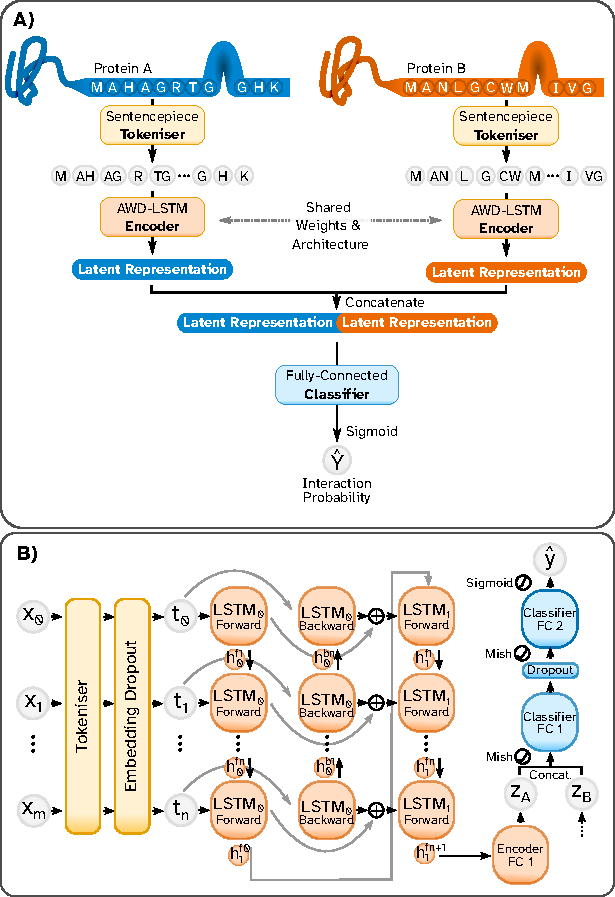
\includegraphics[scale=1]{figures/rapppid/overview_panel.pdf}}
	\caption[Overview of the \textsc{rapppid} pipeline and architecture.]{\textsf{\textbf{Overview of the RAPPPID pipeline and architecture.}} \textbf{(A)} The pipeline of the \textsc{rapppid} begins with two protein sequences. Each sequence is first tokenised by the Sentencepiece tokeniser (yellow). Each sequence of tokens is then inputted separately into an \textsc{awd-lstm} encoder layer which results in a latent representation for each protein. The latent representations of each protein are inputted into a fully-connected classifier layer. The classifier layer outputs the predicted probability of the two proteins interacting. \textbf{(B)} Taking a closer look at the architecture of the \textsc{rapppid}, individual residues $x_0$ to $x_m$ for a protein comprised of $m$ residues are tokenized into $n$ tokens $t_0,t_1,\dots,t_n$. The embedding dropout layer randomly assigns random tokens from the total vocabulary to zero. The encoder layer is comprised of a multi-layer bidirectional \textsc{lstm} whose last hidden state is fed to a fully connected layer before outputting a latent representation $z_A$. $z_A$ is then concatenated with the latent representation of a second protein ($z_b$) before being inputted into the two-layer fully-connected classifier. The output of the classifier is activated by the sigmoid function to produce a probability of interaction.}\label{fig:rapppid:pipeline}
\end{figure}

\subsection{Sequence segmentation and tokenization}

As mentioned earlier, \textsc{rapppid} utilizes the Sentencepiece algorithm (Kudo and Richardson, 2018) to tokenize amino acid sequences. While words form the basis of many natural languages and may break up sentences and phrases into discrete units, no such higher-order segmentation is as immediately apparent in amino acids. Motifs and protein domains possess many analogous qualities to words in natural languages; they appear repeatedly in amino acid sequences and their combination and relative position in these sequences play important roles in the protein structure and function (Anfinsen, 1973). Much like words, however, motifs and protein domains present an `out-of-vocabulary' problem, where unseen examples are difficult to handle. Attempts to solve this problem in natural language processing tasks have resulted in `subword' segmentation algorithms, particularly in difficult-to-segment languages such as Japanese which do not separate words by spaces (Schuster and Nakajima, 2012). Here, we employ the Sentencepiece algorithm (Kudo and Richardson, 2018) to sample tokens from `subword' vocabularies generated by the Unigram algorithm (Kudo, 2018). The Unigram and Sentencepiece algorithms construct vocabularies of arbitrary size by modelling the probabilities of subwords and provides a principled manner for sampling from this distribution to reconstruct sequences. The multi-residue tokens that comprise the vocabulary subdivide low-entropy areas and reduce the overall length of the sequences encoded.

\subsection[Generalizing protein sequence encoding with \textsc{awd-lstm}]{Generalizing protein sequence encoding with AWD-LSTM}

The task of \textsc{ppi} prediction on unseen proteins is a difficult problem prone to overfitting, as demonstrated by the poor testing performance of various methods on unseen proteins (Park and Marcotte, 2012). For this reason, a training and optimization methodology that allows efficient regularization is desirable. \textsc{awd-lstm} was recently devised to enable efficient training of generalizable \textsc{rnn}s (Merity \textit{et al.}, 2017). This approach deploys several regularization techniques during training to achieve this goal. \textsc{rapppid} adopts, with modification, the training methodology of \textsc{awd-lstm}. \textsc{rapppid} utilizes Embedding Dropout, DropConnect (Wan \textit{et al.}, 2013) and Weight Decay (Loshchilov and Hutter, 2019) on the \textsc{lstm} weights, as described by \textsc{awd-lstm}, in the encoder during training. Both \textsc{awd-lstm} and \textsc{rapppid} optimize over average weights; however, the optimizers are quite different. \textsc{awd-lstm} makes use of the \textsc{nt-asgd} optimizer which switches between \textsc{sgd} and the \textsc{asgd} variant. \textsc{rapppid} uses the recent stochastic weight averaging (\textsc{swa}) strategy in combination with the Ranger21 optimizer (Athiwaratkun \textit{et al.}, 2019; Wright and Demeure, 2021). \textsc{swa} has been shown to promote generalizable models in part by overcoming the challenges of finding best solutions within flat loss basins (Izmailov \textit{et al.}, 2019). Ranger21 is an optimizer that applies the `Lookahead mechanism' (Zhang \textit{et al.}, 2019) to the AdamW optimizer (Loshchilov and Hutter, 2019) and includes several optimization techniques (Wright and Demeure, 2021). These techniques, which include gradient centralization and adaptive gradient clipping, enable us to further improve our ability to learn generalized weights and smooth training trajectories (Brock \textit{et al.}, 2021; Yong \textit{et al.}, 2020). Finally, since \textsc{rapppid} does not rely on the timestep outputs of the \textsc{lstm} network, the temporal regularization described by \textsc{awd-lstm} is not applied.

\subsection[Details of \textsc{rapppid}’s architecture and hyper-parameter tuning]{Details of RAPPPID’s architecture and hyper-parameter tuning}

The dimensionality of the \textsc{awd-lstm} hidden state is made equal to the dimensionality of the embeddings (\textit{i.e.}: 64). The output of the fully connected layer is of equal dimensionality to that of the \textsc{awd-lstm} hidden state and is activated by the Mish activation function (Misra, 2020). The output of the first fully connected layer is half the size of the embedding dimension, activated by the Mish function and regularized by a dropout layer (Srivastava \textit{et al.}, 2014). \textsc{rapppid} trains on a vocabulary of 250 tokens that is generated by the Sentencepiece algorithm. New vocabularies are generated for each dataset before training. The number of \textsc{lstm} layers, \textsc{l2} coefficient and various dropout rates are defined as hyper-parameters that require tuning between different datasets. Hyper-parameters were selected by cross-validation. The range of considered hyper-parameters and their selected values are provided in Supplementary Tables \ref{tab:rapppid_hyperparam_range} and \ref{tab:rapppid_hyperparams}. The chosen hyper-parameter ranges are a compromise between common, reasonable values and maintaining a manageable hyper-parameter space which can be explored practically.

\subsection{Protein interaction datasets}

We obtained \textsc{ppi}s and protein sequences from version 11 of the Search Tool for the Retrieval of Interacting Genes/Proteins (\textsc{string}) database (Szklarczyk \textit{et al.}, 2019), from the official \textsc{string} website. Edges were downloaded from \href{https://stringdbstatic.org/download/protein.links.detailed.v11.0.txt.gz}{https://stringdbstatic.org/download/\\protein.links.detailed.v11.0.txt.gz} and sequences were downloaded from \\\href{https://stringdb-static.org/download/protein.sequences.v11.0.fa.gz}{https://stringdb-static.org/download/protein.sequences.v11.0.fa.gz}. In this dataset, the association between any two proteins is assigned a confidence score depending on the source of the information (called a `channel'). In our analyses, only associations with a combined \textsc{string}-score above 95\% (equivalent to a score above 950, obtained from combining different channels) were considered as positive edges. We also retained the channel specific scores for further analysis. To obtain an estimate of the false-positive rate of the confidence score-filtered \textsc{string} dataset, we leveraged the curated and experimentally validated non-interacting protein pairs from the Negatome dataset (Blohm \textit{et al.}, 2014). By comparing the set of proteins that are in both \textsc{string} and Negatome, and evaluating the number of negative edges in Negatome that were considered a positive edge in this intersection, we estimated the false-positive rate of our \textsc{string} dataset to be 4.01\%. This false-positive rate is within the expected 5\% upper-bound given by our 95\% confidence threshold. \textsc{ppi} graphs are understood to be scale-free in the general case. This property of \textsc{ppi} graphs can make them challenging datasets upon which to train a generalized model, as some proteins can be over-represented. To characterize the extent to which proteins are represented in the dataset, we calculated the distribution of the relative degree of proteins in the network (Supplementary Fig. \ref{tab:rapppid_hyperparam_range}A–C). The vast majority of proteins (upwards of 85\%) have edges with fewer than 1\% of proteins within their dataset split (\textit{i.e.}: train/validation/test). The protein with the highest degree is \textit{CDC5L} which has a relative degree of just over 10\%, while the second highest has a relative degree of 6.2\% (Supplementary Fig. \ref{tab:rapppid_hyperparam_range}D–F).

\subsection{Negative examples}

The preparation of datasets of pairs of proteins which are known not to interact with one another is a fraught process. Various methods are typically deployed to create such datasets, which are integral for machine learning methods as they typically require negative examples. Ideally, only negative examples are entirely composed of non-interacting protein pairs which are experimentally verified and manually curated, such as the Negatome database (Blohm \textit{et al.}, 2014).

Unfortunately, non-interacting pairs are difficult to experimentally validate. As a result, there are far fewer \textit{Homo~sapiens} negative protein pairs in such datasets as Negatome than positive protein pairs in databases such as \textsc{string}. Precisely, there are 1~191 negative \textit{H.~sapiens} pairs in Negatome, and 263~130 positive pairs above a 95\% confidence threshold in \textsc{string} (only pairs comprised of proteins present in Uniprot\textsc{kb} were included in this analysis). The resulting class imbalance is detrimental to learning performant, generalizable models.

Synthetic negative pairs are often used to compensate for the small number of experimentally verified non-interacting pairs is construction of synthetic negative pairs. A common method for constructing negative pairs is to select pairs of proteins from distinct sub-cellular compartments. This method has unfortunately been shown to result in biased samples according to multiple measures (Ben-Hur and Noble, 2006). Selecting pairs at random from the space of pairs not known to interact has proven to evade such biases, but runs the risk of capturing yet unknown false negatives. Unless otherwise noted, \textsc{rapppid} utilizes synthetic random pairs of proteins which are not known to interact.

\subsection{Training, validation and testing set construction}

As identified by Park and Marcotte (2012), methods which consider the interaction of proteins in a pairwise fashion must (and have historically failed to) take additional care to avoid information leakage when constructing training and testing datasets. Following their suggestion, here we use three different classes of testing and training sets to evaluate the performance of \textsc{rapppid} and other algorithms (Fig. \ref{fig:rapppid:channels}).

\begin{enumerate}
\item{`\textsc{c1}' refers to the evaluation scheme in which edges (pairs of proteins) are randomly selected to form the training or testing sets. Since the selection criterion is based on edges, both proteins in the pair may be present in both the testing and training sets (due to the presence of other edges adjacent to each protein).}
\item{`\textsc{c2}' refers to the evaluation scheme in which proteins are randomly selected to form the training or testing sets. In this scheme, only one protein in a pair may be present in both testing and training sets (but never both). This evaluation scheme mimics the scenario in which a model trained on the interactome is used to predict the interaction of known proteins with a newly discovered protein (that was not used to train the model).}
\item{`\textsc{c3}' refers to the evaluation scheme in which proteins are randomly selected to form the training or testing sets. However, unlike \textsc{c2}, proteins which appear in the training set never appear in the testing set. This is the most strict evaluation scheme.}
\end{enumerate}

While most methods have typically reported on models validated with datasets in the \textsc{c1} class, they often perform much worse on similar datasets in the more conservative \textsc{c2} and \textsc{c3} classes. This is likely due to the information leakage between training and testing sets present in the \textsc{c1} class and, to a lesser extent, in the \textsc{c2} class. In our evaluations, we report the performance of different methods using all three evaluation schemes above, but we are most interested in the results of \textsc{c3} due to a lack of information leakage. In the C-type datasets we’ve created, there are 9~300 proteins. The number of edges in the datasets ranges from just over 263~000 edges in the \textsc{c1} dataset to just under 174~000 edges in the \textsc{c3} dataset. Full dataset statistics are presented in Supplementary Table \ref{tab:rapppid_data_stats}. These C-type datasets are made freely available to the public through the Zenodo repository at \href{https://doi.org/10.5281/zenodo.6709790}{https://doi.org/10.5281/zenodo.6709790} (Szymborski and Emad, 2022a). We’ve made these datasets available in the hope that it facilitates the evaluation of protein interaction prediction methods on datasets that both mitigate information leakage and are appropriately large for deep learning applications. The adoption of C-type datasets for training and evaluation of \textsc{ppi} prediction methods is important for accurate and representative benchmarking.

\subsection{Implementation}

\textsc{rapppid} was implemented in the Python computer language using the PyTorch and PyTorch Lightning deep learning framework (Falcon \textit{et al.}, 2020; Paszke \textit{et al.}, 2019). Embedding Dropout and DropConnect implementation were obtained from the \textsc{awd-lstm} code base (Merity \textit{et al.}, 2017). The source code for \textsc{rapppid} can be found by visiting \href{https://github.com/jszym/rapppid}{https://github.com/jszym/rapppid} or through the Zenodo repository at \href{https://doi.org/10.5281/zenodo.6709213}{https://doi.org/10.5281/zenodo.6709213} (Szymborski and Emad, 2022b). \textsc{rapppid} was trained at a rate of 2.7 training steps per second at a batch size of 80 protein pairs on an Nvidia \textsc{rtx} 2080 \textsc{gpu} and 32 \textsc{cpu} cores clocked at 2.2 GHz. The \textsc{c3} model takes 2.4 h to train, while \textsc{c1} and \textsc{c2} take 7.8 h.

\begin{figure}[]%figure2
	\centerline{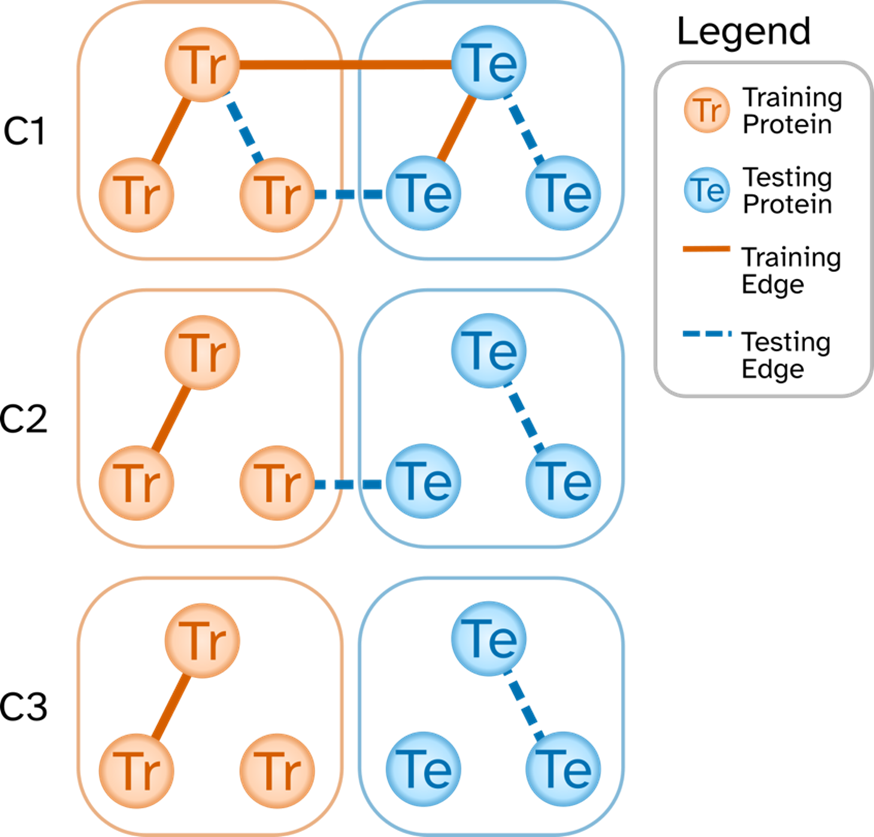
\includegraphics[scale=0.75]{figures/rapppid/c_datasets.png}}
	\caption[Illustration of differences in edges between \textsc{c1}, \textsc{c2}, and \textsc{c3} datasets.]{\textsf{\textbf{Illustration of differences in edges between C1, C2, and C3 datasets.}} Differences between \textsc{c1}, \textsc{c2}, and \textsc{c3} datasets are most visible by first dividing the population of all proteins in the dataset into training (orange, left) and testing (blue, right). In the case of the strict \textsc{c3} dataset (bottom row), edges known at training time (orange, solid) only occur between training proteins. Similarly, \textsc{c3} datasets are evaluated on testing edges (blue, dotted) that only occur between testing proteins. The \textsc{c2} dataset has all the edges present in the \textsc{c3} dataset, but also includes testing edges between testing proteins and training proteins. Finally, the pervasive \textsc{c1} datasets allows all possible training and testing edges that are not identical.}\label{fig:rapppid:c_dataset}
\end{figure}

\subsection{Protein similarity experiments}

In the analysis of the sequence similarity between testing and training proteins, ‘Percent Identity’ was measured between proteins using \textsc{ncbi}’s \textsc{psi-blast} tool running locally as part of version 2.12.0 of \textsc{ncbi}'s \textsc{blast}+ software suite (Altschul \textit{et al.}, 1997). In addition to the Percent Identity, for two proteins to be considered similar, an E-value cut-off of at most 5 and an alignment length of more than 30\% of the query sequence were considered necessary. The 64-bit Linux binaries of the \textsc{blast}+ suite were obtained from the link \\\href{ftp://ncbi.nlm.nih.gov/blast/executables/blast+/2.12.0/}{ftp://ncbi.nlm.nih.gov/blast/executables/blast+/2.12.0/}.

\section{Results}

\subsection[Performance evaluation of \textsc{rapppid} and other algorithms]{Performance evaluation of RAPPPID and other algorithms}

To establish the ability of \textsc{rapppid} to correctly predict \textsc{ppi}s within the current landscape of \textsc{ppi} prediction methods, we compared it against three recent methods (Fig. \ref{fig:rapppid:auroc}). The first of these is the Scoring Protein INTeractions (\textsc{sprint}) method, which belongs to the family of methods that predict interactions according to measures of sequence similarity (Li and Ilie, 2017). \textsc{sprint} was shown to outperform \textsc{svm}, random forest and sequence similarity-based methods across \textsc{c1}, \textsc{c2} and \textsc{c3}-like datasets.

The two other methods, \textsc{pipr} and Deep\textsc{ppi}, are deep learning methods that similar to \textsc{rapppid} utilize twin networks (Chen \textit{et al.}, 2019; Richoux \textit{et al.}, 2019). \textsc{pipr} uses a residual recurrent convolutional neural network for its encoder with the goal of more effectively summarizing both local and global features. We compared \textsc{rapppid} against the best performing iteration of Deep\textsc{ppi}, whose encoder comprises of a convolutional neural network feature extractor followed by an \textsc{lstm} network. All three methods required retraining, as the available weights of these models belong to diverse datasets, all of which are either not \textsc{c2} or \textsc{c3} type, or (in the case of \textsc{sprint}) are insufficiently large for training a generalized deep learning model. Across \textsc{c1}, \textsc{c2} and \textsc{c3} testing datasets, \textsc{rapppid} achieved higher area under the receiver-operator curve (\textsc{auroc}) than all other methods tested (Table~\ref{Tab:auroc}). The margin between \textsc{rapppid} and the second highest performing method (\textsc{sprint} in all cases) was highest when performed on the stricter \textsc{c3} dataset, resulting in 24.3\% improvement. The improvement obtained by \textsc{rapppid} compared to \textsc{sprint} was lower on the \textsc{c2} dataset (3.4\%), and finally nearly equivalent on the least strict \textsc{c1} dataset. With regards to the area under the precision-recall curve (\textsc{aupr}), this trend across dataset types persisted. \textsc{rapppid}’s \textsc{aupr} was higher than all other methods for the \textsc{c3} dataset, with a margin to the second highest method of 0.094 (equivalent to a 14.6\% improvement). \textsc{rapppid}’s \textsc{aupr} score was matched by \textsc{sprint} in experiments conducted on the \textsc{c2} dataset, but outperformed Deep\textsc{ppi} and \textsc{pipr}. \textsc{sprint} achieved the highest \textsc{aupr} of all the methods in the \textsc{c1} dataset, outperforming \textsc{rapppid} with a margin of 0.009 (equivalent to a 0.9\% improvement). 

\begin{table}[!t]
	\caption[Comparison of \textsc{ppi} prediction performance on \textsc{c1}, \textsc{c2}, and \textsc{c3} datasets.]{\textbf{\textsf{Comparison of PPI prediction performance on C1, C2, and C3 datasets.}}
    \label{tab:rapppid:auroc}} {
    \begin{center}
    \begin{tabular}{@{}llll@{}}\toprule 
			Dataset & Method & Testing \textsc{auroc} & Testing \textsc{aupr}\\\midrule
			\textsc{c1} & \textsc{rapppid} & \textbf{0.978} & 0.974\\
			    & \textsc{sprint} & 0.977 & \textbf{0.983}\\
			    & Deep\textsc{ppi} & 0.874 & 0.881\\
			    & \textsc{pipr} & 0.501 & 0.405\\\midrule
			\textsc{c2} & \textsc{rapppid} & \textbf{0.859} & \textbf{0.868}\\
			   & \textsc{sprint}  & 0.830 & \textbf{0.868}\\
			   & Deep\textsc{ppi} & 0.760 & 0.787\\
			   & \textsc{pipr} & 0.507 & 0.508\\\midrule
			\textsc{c3} & \textsc{rapppid} & \textbf{0.803} & \textbf{0.810}\\
			   & \textsc{sprint}  & 0.646 & 0.716\\
			   & Deep\textsc{ppi} & 0.574 & 0.590\\
			   & \textsc{pipr} & 0.505 & 0.509\\
			\midrule
	\end{tabular}
    \\\\
    {\footnotesize Note: The testing AUROC and AUPR of four different PPI prediction methods is reported across the three different dataset types described by Park and Marcotte (Park and Marcotte, 2012). The highest value for each dataset are reported in boldface.}
    \end{center}
    }{}
\end{table}

While we were able to replicate results of the \textsc{pipr} model on the \textit{Saccharomyces cerevisiae} dataset published as part of the original \textsc{pipr} publication (Chen \textit{et al.}, 2019), \textsc{pipr} suffered from convergence issues during training on our \textit{H.~sapiens} \textsc{string} datasets. We suspect this is due to a variety of factors, with the large differences in dataset characteristics being the most likely cause. The number of proteins and interactions in the \textit{S. cerevisiae} dataset is far smaller than our \textsc{string} datasets. Furthermore, the \textit{S. cerevisiae} dataset selected pairs of proteins which occupy different sub-cellular compartments in order to construct negative samples; an approach found to lead to biased estimations of prediction accuracy (Ben-Hur and Noble, 2006). Taken together, these results suggest that \textsc{rapppid} outperforms alternative methods in the majority of evaluations on \textsc{c1}, \textsc{c2} and \textsc{c3} schemes and is particularly effective in the stricter and more difficult \textsc{c3} evaluation.

\begin{figure*}[b!]%figure3
	\centerline{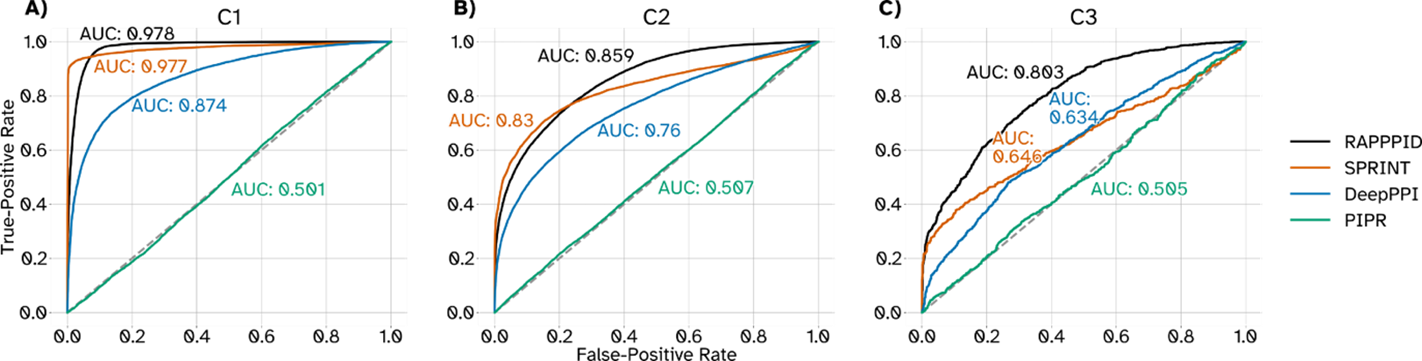
\includegraphics[scale=0.9]{figures/rapppid/auroc.png}}
	\caption[Receiver-Operator curves across methods and datasets.]{\textsf{\textbf{Receiver-Operator curves across methods and datasets.}} The receiver-operator curves (\textsc{roc}s) for all four methods tested across \textsc{c1} \textbf{(A)}, \textsc{c2} \textbf{(B)}, and \textsc{c3} \textbf{(C)} datasets.}\label{fig:rapppid:auroc}
\end{figure*}

\subsection[Channel-specific performance of \textsc{rapppid}]{Channel-specific performance of RAPPPID}

The \textsc{string} database, integrates and annotates protein association data from a wide range of sources. The `database', `text-mining', `experiments' and `co-expression' channels make up the majority of the edges in our datasets (\textit{e.g.}: 98.4\% of all the edges in the \textsc{c3} dataset). The `database' channel is comprised of several curated databases of interactions such as \textsc{kegg} and Reactome (Jassal \textit{et al.}, 2019; Kanehisa and Goto, 2000). Edges in the `text-mining' channel are the result of a statistical analysis of proteins whose names and/or identifiers co-occur in publications. The `experiments' channel is populated by interactions evidenced by high-throughput experiments curated by members of the International Molecular Exchange (\textsc{ime}x) consortium (Orchard \textit{et al.}, 2012). This includes datasets such as IntAct, \textsc{dip}, the Bio\textsc{grid} and many others (Orchard \textit{et al.}, 2014; Oughtred \textit{et al.}, 2021; Salwinski \textit{et al.}, 2004). Finally, the `coexpression' channel arises from proteomic and transcriptomic assays which quantify gene-by-gene correlations. \textsc{string} additionally assigns calibrated confidence scores to each of the edges which summarize the evidence supporting an edge. Scores are assigned to each edge by channel, and finally harmonized into a final ‘combined confidence score’ which represents the evidence across all channels present in ‘\textsc{string}’. To better characterize the results of our protein-protein prediction tests, we sought to identify the source of the testing edges \textsc{rapppid} correctly and incorrectly identified. Figure \ref{fig:rapppid:channels}A and Supplementary Figure \ref{fig:rapppid:channels_supp} show that \textsc{rapppid} can accurately predict the testing set edges that have a high confidence score in biologically supported channels of co-expression, experiments, and database. However, the accuracy for the edges that have a high confidence score in the text-mining channel is inferior to the other channels. Since edges that are only supported by text-mining (but not by the other channels) are arguably the ones most prone to error, we expected \textsc{rapppid} to have an inferior performance on such edges (since the edges themselves may not be reliable). To test whether the inferior performance of \textsc{rapppid} in the text-mining channel in Figure \ref{fig:rapppid:channels}A is indeed due to such edges, for a fixed threshold $k$ ($50\leq k \leq 95$), we divided the testing edges with a text-mining confidence score at least equal to $k$ into two groups: a group with `experiments' confidence score at least equal to 80\% and a group with `experiments' confidence score smaller than 80\% (Fig. \ref{fig:rapppid:channels}B). Evaluating the testing edges in \textsc{c1}, \textsc{c2} and \textsc{c3} showed that for this channel, the accuracy on the former group is higher than the latter group (sometimes as large as 22\% higher, Supplementary Fig. \ref{fig:rapppid:channels_supp2}). Repeating the analysis for co-expression and database channels also confirmed this trend (Fig. \ref{fig:rapppid:channels}B and Supplementary Fig. \ref{fig:rapppid:channels_supp2}). Taken together, these results suggest that the inferior performance of \textsc{rapppid} on the text-mining channel in Figure \ref{fig:rapppid:channels}A is indeed due to the edges that are supported only by text-mining and not by other biologically identified channels.

\begin{figure}[h!]%figure4
	\centerline{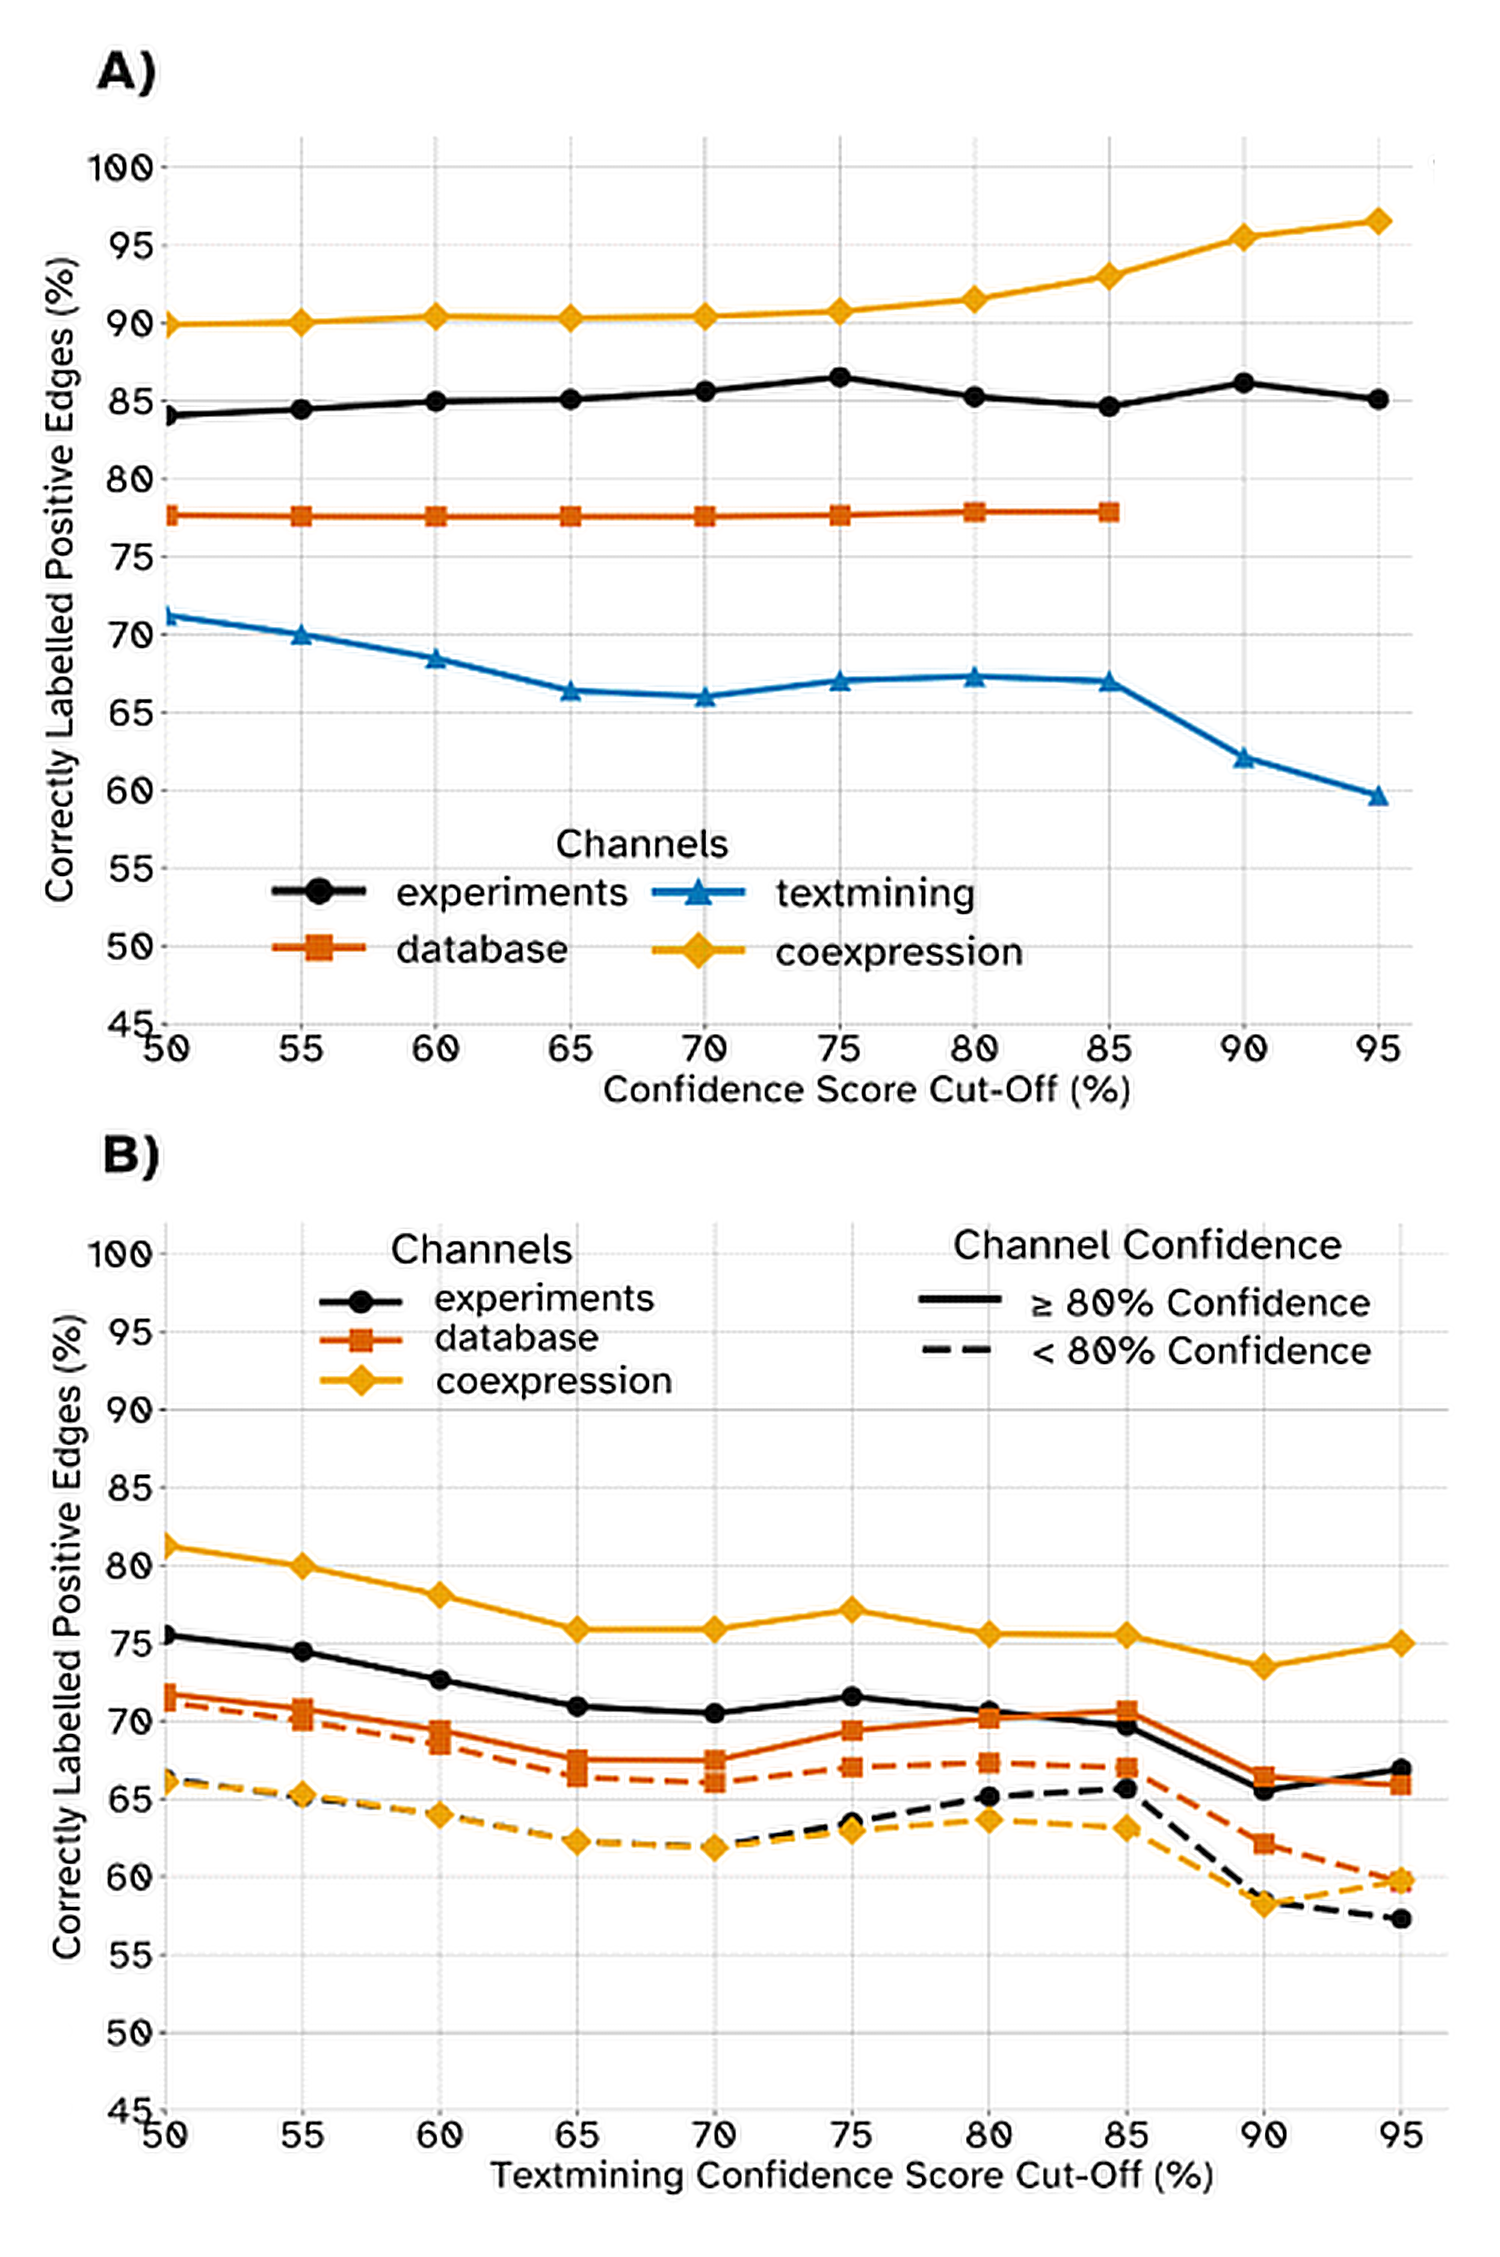
\includegraphics[scale=0.5]{figures/rapppid/channels.png}}
	\caption[Accuracy of positive edges across edge confidence stratified by \textsc{string} channels.]{\textsf{\textbf{Accuracy of positive edges across edge confidence stratified by \textsc{string} channels.}} \textbf{(A)} The percentage of correctly labelled positive edges are plotted for each major \textsc{string} channel. The x-axis denotes the channel edge confidence cut-off score for each curve’s respective channel. \textbf{(B)} Here, we see a similar chart but rather than using each channel’s respective score as a confidence cut-off, edges are excluded according to their text-mining confidence (x-axis). The solid curves include edges which have a channel confidence \hbox{$\geq$80\%}  for the channel indicated by the curve’s colour. Dashed curves conversely include edges whose channel confidence is 80\% for the channel indicated by the curve’s colour.  In both \textbf{(A)} and \textbf{(B)} data shown reflects the \textsc{c2} model/dataset.}\label{fig:rapppid:channels}
\end{figure}

\subsection[Role of protein similarity on \textsc{rapppid}’s performance]{Role of protein similarity on RAPPPID’s performance}

The procedures for \textsc{c2} and \textsc{c3} datasets were devised to reduce the information leakage by avoiding testing on edges which contain proteins which are known to an algorithm during its training. This safeguard against information leakage, however, does not account for proteins which are known by different identifiers but share near identical protein sequences. Further complicating the matter, sequence similarity is a valid \textsc{ppi} prediction feature and is often used by methods as a proxy measure of co-evolution and conserved functional domains (Cong \textit{et al.}, 2019; Jansen, 2003). Indeed, this strategy is leveraged by the \textsc{sprint} algorithm against which \textsc{rapppid} was compared.

In spite of the challenges above, we sought to determine whether the superior performance of \textsc{rapppid} (particularly in the strict datasets of \textsc{c2} and \textsc{c3}) is due to sequence similarity between testing and training proteins or not. For this purpose, we used \textsc{psi-blast} algorithm (Altschul \textit{et al.}, 1997) to evaluate sequence similarities between each pair of testing/training proteins. Figure \ref{fig:rapppid:similarity} shows the accuracy of \textsc{rapppid} on the \textsc{c2} dataset when different degrees of restriction on sequence similarity are imposed. More specifically, a threshold $t$ (x-axis in Fig. \ref{fig:rapppid:similarity}) determined the maximum allowable Percent Identity score between a testing protein and any of the training proteins that were candidates to be similar to it (see Section~\ref{sec:rapppid:methods} for details). Any testing protein that did not satisfy this condition for the threshold t was excluded from the calculation of accuracy. As one moves towards larger values of $t$, the sequence similarity constraint loosens and $t = 100\%$ is equivalent to the complete \textsc{c2} dataset. Our analysis of \textsc{c2} (Fig. \ref{fig:rapppid:similarity}) and \textsc{c3} (Supplementary Fig. \ref{fig:rapppid:similarity_supp}) revealed that \textsc{rapppid}’s accuracy is largely independent of the sequence similarities between testing and training proteins and the performance of \textsc{rapppid} does not deteriorate when removing testing proteins that have a highly similar training protein.

\begin{figure}[h!]%figure4
	\centerline{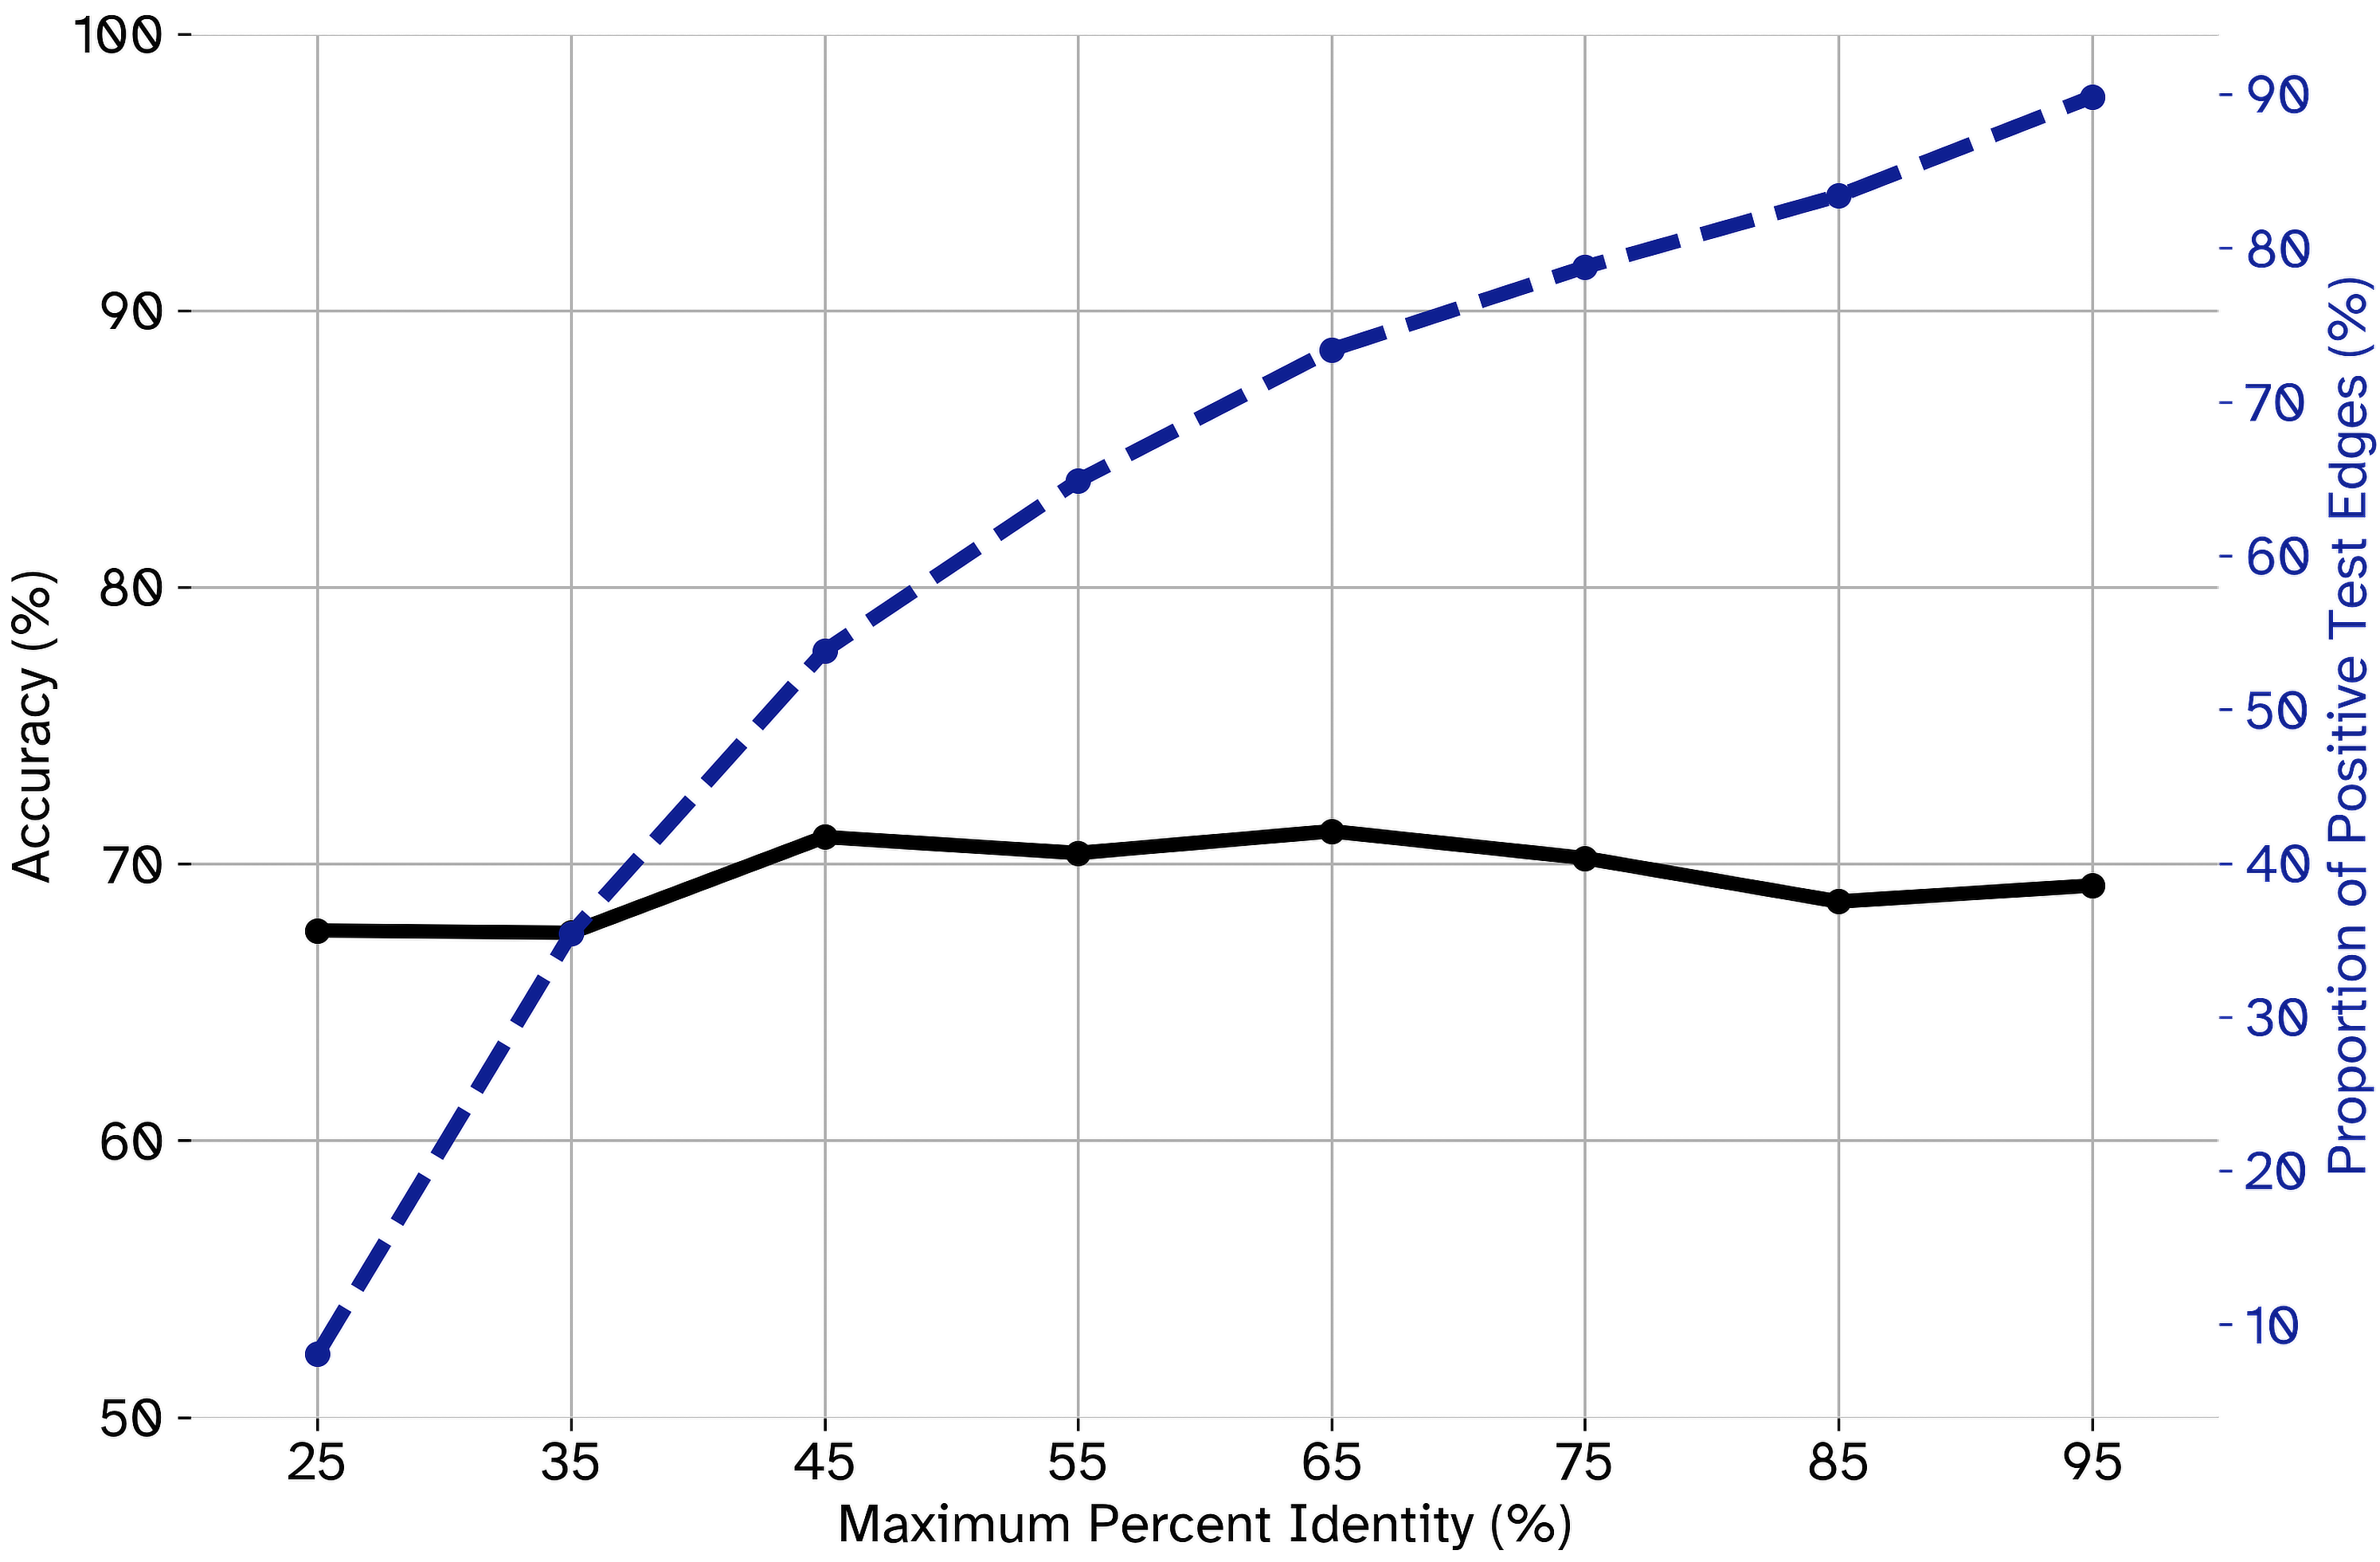
\includegraphics[scale=0.5]{figures/rapppid/perc_id.png}}
	\caption[Accuracy of positive edges as a function of similarity between testing and training proteins in \textsc{c2}.]{\textsf{\textbf{Accuracy of positive edges as a function of similarity between testing and training proteins in C2.}} The similarity between testing and training proteins was measured using their percent identity as computed by \textsc{ncbi}’s \textsc{psi-blast} software. The highest percent identity between any training protein and a testing protein in a testing edge was considered to be that testing edge’s ``maximum percent identity''. The percentage of accurately labelled positive edges (black curve, left y-axis) is reported for edges with maximum percent identities lower than the threshold reported on the x-axis. The proportion of testing edges for each threshold values is reported by the dashed blue curve and the right y-axis.}\label{fig:rapppid:similarity}
\end{figure}

\subsection[Effect of different components on \textsc{rapppid}'s performance]{Effect of different components on RAPPPID's performance}

To understand \textsc{rapppid}’s performance when trained and tested on negative examples which are experimentally validated and manually curated, we created a new C3 dataset where the negative examples are provided by the Negatome database of non-interacting pairs. To combat the large class imbalance caused by the relatively few pairs of human proteins in Negatome (see Section~\ref{sec:rapppid:methods} for details), additional random pair negatives were supplemented until both positive and negative classes had an equal number of samples. After 13 epochs, \textsc{rapppid} achieved a testing \textsc{auroc} of 0.802 and a testing \textsc{aupr} of 0.799 on \textsc{c3} dataset, which is comparable to the performance of \textsc{rapppid} using randomly selected negative edges. Since \textsc{rapppid} utilizes random initialization, mini-batch sampling, and token sampling, there is some stochasticity present in its performance. First, we sought to test the effect of these stochastic components and to ensure that the specific choice of training and test sets were not responsible for the superior performance of \textsc{rapppid}. For this purpose, we ran \textsc{rapppid} twice on three additional \textsc{c3} datasets whose training, validation, and testing proteins were chosen at random (a total of six times). In each of these runs, different seeds were used to assess the effect of stochastic components of \textsc{rapppid} (Supplementary Table \ref{tab:rapppid_repeatability}). Overall, the average testing \textsc{auroc} across models trained on these additional three datasets was 0.792 (60.007). Results from these repeatability experiments illustrate that \textsc{rapppid}’s strong performance on \textsc{c3} datasets is not tied to a specific set of testing or validation proteins, nor certain weight initialization states. Next, we conducted an ablation study (Table~\ref{tab:ablation}) using the same three \textsc{c3} datasets and two runs of each variant per dataset (a total of six models per variant). Each variant substitutes one component of \textsc{rapppid}’s regularization, architecture or optimization, allowing us to quantify the difference in performance for which these components are responsible. In Table 2, `\textsc{rapppid-swa}' variant removes \textsc{swa}, `\textsc{rapppid}+Adam' replaces Ranger21 with Adam optimizer (learning rate selected by hyper-parameter tuning), `\textsc{rapppid-awd}' removes the \textsc{awd} regularization and `\textsc{rapppid}-SentencePiece’ substitutes the SentencePiece tokens with amino-acid-residue-level tokens. As can be seen in Table 2, the choice of optimizer has negligible effect on the performance. However, \textsc{swa}, \textsc{awd}, and SentencePiece tokens all contribute to the superior performance of \textsc{rapppid}, with the tokenizer having the largest contribution. One advantage that SentencePiece affords \textsc{rapppid} is the regularizing effect of random sampling tokens. Additionally, the SentencePiece tokenizer reduces the total length of sequences inputted into the tokenizer. The protein sequences on which \textsc{rapppid} is trained, while limited to 1~500 residues, are sufficiently large enough for gradients to vanish quiet substantially; a phenomenon long known to plague \textsc{rnn}s when trained on long sequences.

\begin{table}[!t]
	\caption[Results from an ablation study conducted on \textsc{rapppid}.]{\textsf{\textbf{Results from an ablation study conducted on RAPPPID.}} \label{tab:ablation}} {\begin{tabular}{@{}lllll@{}}\toprule 
			Experiment & Test \textsc{auroc} & \textsc{auroc} Diff & Testing \textsc{apr} & \textsc{apr} Diff\\\midrule
			\textsc{rapppid} (original) & 0.792 (±0.007) & \textsc{n/a} & 0.794 (±0.009) & \textsc{n/a}\\
			\textsc{rapppid-swa} & 0.782 (±0.007) & -1.20\% & 0.783 (±0.007) & -1.37\%\\
			\textsc{rapppid}+Adam & 0.791 (±0.025) & -0.100\% & 0.792 (±0.032) & -0.273\%\\
			\textsc{rapppid-awd} & 0.762 (±0.020) & -3.70\% & 0.757 (±0.022) & -4.62\%\\
			\textsc{rapppid}-SentencePiece & 0.749 (±0.009) & -5.37\% & 0.748 (±0.011) & -5.85\%\\
			\textsc{rapppid}+TransfLG & 0.670 (±0.030) & -15.3\% & 0.686 (±0.040) & -13.6\%\\
			\textsc{rapppid}+TransfSM & 0.747 (±0.026) & -5.68\% & 0.758 (±0.025) & -4.61\%\\
			\midrule
	\end{tabular}}{}
    \\
    {\footnotesize Note: Each model is trained/tested twice on three randomly generated C3 datasets.\\The performance metrics correspond to held-out test sets.}
\end{table}

In acknowledgement of the recent prevalence and performance of attention-based methods in deep learning (Vaswani \textit{et al.}, 2017), the sixth and seventh variants replace the \textsc{awd-lstm} encoder with transformers of varying sizes. `\textsc{rapppid}+TransfLG' has six layers and eight heads and feed-forward networks with 2048 dimensions, while `\textsc{rapppid}+TransfSM'’ has fewer parameters (2 layers, 2 heads and 80 dimensions). Both transformer variants have a dropout rate of 20\%. The number of heads and layers in \textsc{rapppid}+TransfLG were chosen to closely match those used in the \textsc{bert} language model (Devlin et al., 2019) whose architecture has been previously used for predicting protein function (Elnaggar \textit{et al}., 2021; Rao \textit{et al.}, 2020; Rives \textit{et al.}, 2019). The number of heads and layers for \textsc{rapppid}+TransfSM were chosen to be representative of reasonable lower bounds for those hyperparameters. The results of these analyses (Table 2) reveal that both of these models have worse performance compared to the original \textsc{rapppid} model. The superior performance of the small transformer compared to the large one suggests that the large number of parameters required by transformers are leading to severe overfitting in this task and are the reason behind the performance deterioration.

\subsection{Transfer learning on protein-ligand data from X-ray crystallography experiments}

\textsc{rapppid}'s strong performance on \textsc{c3} datasets demonstrates that it is capable of generalizing to predictions between proteins absent from the training set. Additionally, the ability to generalize these models to make predictions on test datasets that are not representative of the training data (\textit{e.g.} different types of experiments or protocols are used to generate them) is also often desirable, yet is often much more challenging. Transfer learning is one approach that can be used to overcome the challenges imposed by differences between training and test datasets. Transfer learning is the process by which a network is first trained on a large, high-quality dataset. Many of these weights are then `frozen' such that they are no longer backpropagated through, while the remaining `unfrozen' weights are trained on a dataset that is often smaller and/or belongs to a different input distribution (Yosinski \textit{et al.}, 2014). Here, we use this approach to tackle an interaction prediction task on a dataset that differs fundamentally from \textsc{string}: protein-ligand interactions and sequences as determined from X-ray crystallography data. \textsc{string} and similar \textsc{ppi} datasets curate interactions from a wide range of modalities and provide sequences from reference proteomes. We’ve constructed a protein-ligand interaction task by leveraging BioLiP, a semi-manually curated list of X-ray crystallography experiments recorded in the Protein Data Bank (\textsc{pdb}) which reflect interactions between proteins and ligands (Berman \textit{et al.}, 2000; Yang \textit{et al.}, 2013). Using these datasets, we were able to extract sequences from the \textsc{pdb} records and, after filtering out interactions with low-quality sequences, construct a novel protein-ligand dataset. This dataset is available for download through Zenodo at \href{https://doi.org/10.5281/zenodo.6709790}{https://doi.org/10.5281/\\zenodo.6709790} (Szymborski and Emad, 2022a). The sequences extracted from \textsc{pdb} are measured by fundamentally different modalities from those present in \textsc{string}/Uniprot\textsc{kb}, and are often truncated and incomplete as a result. Furthermore, the nature of the interactions recorded by BioLiP is fundamentally different from \textsc{string}. Whereas \textsc{string} catalogues interactions between large classes of proteins, the nature of X-ray crystallography biases captured interactions to those with slower molecular dynamics and which do not primarily exist in aliphatic environments (Carpenter et al., 2008). These fundamental differences between BioLiP and \textsc{string} make them ideal datasets to illustrate the ability to use transfer learning with \textsc{rapppid}. We first pre-trained \textsc{rapppid} on data from \textsc{string}, and then fine-tuned it on the BioLiP dataset after the \textsc{lstm} encoder weights were frozen, leaving only the fully connected classifier to be trained. To ensure no data leakage between the \textsc{string} and BioLiP datasets exists, protein sequences in \textsc{string} determined to have more than 90\% identity with those in BioLiP were moved from the pre-training dataset to the fine-tuning dataset. \textsc{c3}-type training, validation and testing splits were constructed for both the pre-training and finetuning datasets for evaluation purposes. Using this approach, \textsc{rapppid} pre-trained on the \textsc{string} dataset and fine-tuned on a portion of the BioLip dataset achieved an \textsc{auroc} of 0.909. To test our hypothesis that transfer learning is indeed necessary to achieve good performance on this dataset, we also directly applied the pretrained \textsc{rapppid} model (without any fine-tuning on BioLip) to the BioLip test split. As expected, this resulted in almost random results (\textsc{auroc} = 0.548). These results highlight the difficulties of generalizing a model to fundamentally different datasets and emphasise the utility of transfer learning to achieve good performance using \textsc{rapppid} in such scenarios.

\subsection[\textsc{rapppid} predicts interaction of \textsc{her2} with Trastuzumab and\\Pertuzumab]{RAPPPID predicts interaction of HER2 with Trastuzumab and\\Pertuzumab}

Peptides and proteins have emerged as an important class of therapeutics, enabling researchers to target previously `undruggable' targets (Tsomaia, 2015). Hundreds of peptide and protein therapeutics have been approved by the \textsc{u.s.} Food and Drug Administration (Usmani \textit{et al.}, 2017) with applications in treating illnesses ranging from cancer to heart disease (Chen \textit{et al.}, 2012; Sikder \textit{et al.}, 2019). Here, we sought to illustrate how one might use \textsc{rapppid} to validate hypothesized interactions between target proteins and candidate therapeutic proteins and peptides through two examples: Trastuzumab and Pertuzumab. Trastuzumab and Pertuzumab are two recombinant humanized monoclonal antibodies which are used in combination in the treatment of metastatic breast cancers which belong to the \textsc{her2}-positive subtype (Boekhout \textit{et al.}, 2011; Malenfant \textit{et al.}, 2014). Both Trastuzumab and Pertuzumab target distinct domains of the human epidermal growth factor receptor 2 (\textsc{her2}). We applied \textsc{rapppid}, trained on our \textit{H.~sapiens} \textsc{string} \textsc{c2} dataset (which is more appropriate for this application), to the sequences of the Trastuzumab and Pertuzumab antibody chains. \textsc{rapppid} predicted that \textsc{her2} interacts with Trastuzumab and Pertuzumab with 98.8\% and 95.1\% probability, respectively. When compared to the interaction probabilities between these drugs and all other proteins in the \textsc{string} database, these probabilities are within the first and second percentile for Trastuzumab and Pertuzumab, respectively (Supplementary Fig. \ref{fig:rapppid:trastuzumab}). In addition, the majority of proteins are predicted to have a probability of interacting with Trastuzumab and Pertuzumab of 35.9\% and 28.8\%, respectively.

\section{Discussion}

This study introduced \textsc{rapppid}, a deep learning method that addresses the challenges of creating generalizable \textsc{ppi} prediction models posed by inherent characteristics of \textsc{ppi} datasets. By adopting a modified \textsc{awd-lstm} training routine, \textsc{rapppid} was able to surpass state-of-the-art models under testing conditions that carefully controlled for information leakage and other sources of prediction accuracy inflation. Further experiments were conducted to confirm the results were independent of the specific proteins present in the training and testing splits. \textsc{rapppid}s ability to \textsc{ppi}s in the \textsc{string} database was shown to increase with strong biological evidence for the interaction. This relationship between \textsc{ppi} evidence and \textsc{rapppid} predictive ability illustrates that \textsc{rapppid} accurately reflects our confidence in interactions, and testing performance is not disproportionately inflated by spurious, low-confidence interactions. Moreover, assessment of the sequence similarity between testing and training proteins revealed that the superior performance of \textsc{rapppid} is not due to the presence of highly similar protein pairs in testing and training, and the accuracy of \textsc{rapppid} was largely stable with a small improvement when highly similar testing proteins were excluded. Developing appropriate and meaningful benchmark datasets for \textsc{ppi} prediction remains a challenging problem for a number of reasons. First, deep learning tasks rely on large, high-quality datasets to obtain meaningful generalized models. Such datasets are few and far between. Projects like \textsc{hippie} and iRefWeb join \textsc{string} in being among the best examples of \textsc{ppi} datasets which integrate multiple sources to assure both quality and quantity of \textsc{ppi} edges (Alanis-Lobato \textit{et al.}, 2017; Turner \textit{et al.}, 2010). Despite this, \textsc{string} is the only dataset among these three which has an appropriate number of high-confidence edges for the purpose of learning deep learning model. Specifically, there are 98.5\% fewer edges in \textsc{hippie} than in \textsc{string} between human proteins at a 95\% confidence threshold. Even when confidence thresholds are lowered to 85\%, \textsc{hippie} holds 87.9\% fewer human edges than \textsc{string}. Similarly, \textsc{string} at a 95\% confidence threshold has 75\% more human edges when considering iRefWeb edges with three supporting references or more. Second, this reliance on large, representative datasets is further exacerbated by the unique overfitting challenges posed by the characteristics of \textsc{ppi} data, as explored in this work and in Park and Marcotte (Park and Marcotte, 2012). While \textsc{rapppid} mitigates the overfitting tendencies of \textsc{ppi} data through regularization, it also relies on large, representative training data to do so. In the construction of our \textsc{c3} datasets, it is necessary to discard edges which are not between proteins of the same validation split. As a result, we observe a further decrease of up to 33.9\% in the number of the already-precious-few edges afforded to us by \textsc{string}. As we have shown in this work, the construction of benchmark datasets is critical for effectively comparing and evaluating \textsc{ppi} prediction tasks. It is thanks to large, quality \textsc{ppi} dataset projects like \textsc{string} that we might construct meaningful and appropriate datasets against which to evaluate \textsc{ppi} prediction methods like \textsc{rapppid}. Additional efforts and methodologies to collect and integrate \textsc{ppi} edges of the scale of \textsc{string} at high confidence levels are greatly desired, as they can help identify and mitigate biases that inevitably arise when constructing datasets. In our analysis, we observed that \textsc{rapppid} assigns a very high probability of interaction to \textsc{her2} and Trastuzumab (first percentile) and Pertuzumab (second percentile). In spite of this, there are still proteins that are predicted by \textsc{rapppid} to interact with these two antibodies with similar or higher probabilities (72 for Trastuzumab and 206 for Pertuzumab). This of course is not unique to \textsc{rapppid} and other methods also face this issue to an even a greater extent. For example, \textsc{sprint} (the second-best performing algorithm after \textsc{rapppid}) assigns a higher interaction score to 389 proteins for Trastuzumab-\textsc{her2} and 456 proteins for Pertuzumab-\textsc{her2}. We believe there are several factors contributing to this. First, all of these methods face some limitations in their performance, as we explored and observed in our cross-validation analyses. Second, there are off-target effects of these antibodies that make the prediction challenging for these computational models. Finally, there may be domain shifts between the interacting proteins in \textsc{string} dataset and the interaction of these antibodies and their targets, a similar phenomenon that we observed in BioLiP dataset. This suggests that transfer learning approaches such as the one we used for BioLiP dataset may be useful to improve the specificity of these algorithms, a direction that we will pursue in the future. As a result of these factors, while \textsc{rapppid} can be used to narrow down the search space of novel therapeutic antibodies and peptides, it does not remove the necessity of follow-up experimental validations to identify their targets. The task of \textsc{ppi} prediction is related to the problem of protein docking inference, whereby computational models predict the atomic interactions between two proteins. While many methods have historically been based on the fast Fourier transform for energy evaluation (Desta \textit{et al.}, 2020), new and effective deep learning methods have also become available. One such method is AlphaFold-multimer (Evans \textit{et al.}, 2021), which builds upon an attention-based model for the prediction of protein structure (Jumper \textit{et al.}, 2021) to infer the interface of homo and hetero protein dimers at an atomic level. Integrating docking predictions can be an interesting future direction to help improve \textsc{rapppid}’s \textsc{ppi} prediction generalization. \textsc{rapppid}’s ability to predict interactions warrants further study into relevant tasks that might benefit from a similar approach. The \textsc{rapppid} architecture might be modified for the tasks of binding site and protein function prediction. These tasks are related to \textsc{ppi} prediction and as a result are exposed to similar challenges to which \textsc{rapppid} is well suited. While our ablation studies found that \textsc{rapppid} using a Transformer architecture for the encoder performed worse than an \textsc{awd-lstm}, using a Transformer model pre-trained on amino acid sequences might improve performance. However, in all these cases, it is crucial to consider strict rules for cross-validation and data splitting to ensure data leakage is avoided.

\section*{Authors' contributions}
\addcontentsline{toc}{section}{Authors' contributions}

\textsc{a.e.} and \textsc{j.s.} conceived the study, designed the project and the algorithm, and wrote the article. \textsc{j.s.} implemented the pipeline and performed the statistical analyses of the results. All authors read and approved the final article.

\section*{Funding}
\addcontentsline{toc}{section}{Funding}

This work was supported by the Natural Sciences and Engineering Research Council of Canada (\textsc{nserc}) grant [\textsc{rgpin}-2019-04460 to \textsc{a.e.}] and by the McGill Initiative in Computational Medicine (MiCM) (to \textsc{a.e.}). This research was enabled in part by support provided by Calcul Qu\'ebec (\href{https://www.calculquebec.ca/}{www.calculquebec.ca}) and Compute Canada (\href{https://www.computecanada.ca}{www.computecanada.ca}).

\section*{Data availability}
\addcontentsline{toc}{section}{Data availability}

The data underlying this article are available on Zenodo.org, at \href{https://doi.org/10.5281/zenodo.6709790}{https://doi.org/10.5281/zenodo.\\6709790}.

\begin{singlespace}
\def\bibindent{1em}
\makeatletter
\renewcommand{\thebibliography}[1]{%
  \section*{\bibname}%
  \addcontentsline{toc}{section}{References}
  \@mkboth{\MakeUppercase\bibname}{\MakeUppercase\bibname}%
  \list{\@biblabel{\@arabic\c@enumiv}}%
       {\settowidth\labelwidth{\@biblabel{#1}}%
        \leftmargin\labelwidth
        \advance\leftmargin\labelsep
        \@openbib@code
        \usecounter{enumiv}%
        \let\p@enumiv\@empty
        \renewcommand\theenumiv{\@arabic\c@enumiv}}%
  \sloppy
  \clubpenalty4000
  \@clubpenalty \clubpenalty
  \widowpenalty4000%
  \sfcode`\.\@m}
\makeatother
\renewcommand{\bibname}{References}
\begin{thebibliography}{99\kern\bibindent}
\markboth{Chapter 3: \textsc{rapppid}}{Chapter 3: \textsc{rapppid}}
\makeatletter
\def\@biblabel#1{}
\let\old@bibitem\bibitem
\def\bibitem#1{\old@bibitem{#1}\leavevmode\kern-\bibindent}
\makeatother
\bibitem{Lorem}Alanis-Lobato,G. \textit{et al.} (2017) Hippie v2.0: enhancing meaningfulness and reliability of protein–protein interaction networks. \textit{Nucleic Acids Res.}, 45, D408–D414.
\bibitem{Lorem}Altschul,S.F. \textit{et al.} (1990) Basic local alignment search tool. \textit{J. Mol. Biol.}, 215, 403–410.
\bibitem{Lorem}Altschul,S.F. \textit{et al.} (1997) Gapped BLAST and PSI-BLAST: a new generation of protein database search programs. \textit{Nucleic Acids Res.}, 25, 3389–3402.
\bibitem{Lorem}Anfinsen,C.B. (1973) Principles that govern the folding of protein chains. \textit{Science}, 181, 223–230.
\bibitem{Lorem}Athiwaratkun,B. \textit{et al.} (2019) There are many consistent explanations of unlabeled data: Why you should average. In: \textit{7th International Conference on Learning Representations, ICLR 2019, New Orleans, LA, USA, May 6-9, 2019}. OpenReview.net.
\bibitem{Lorem}Ben-Hur,A. and Noble,W.S. (2005) Kernel methods for predicting protein-protein interactions. \textit{Bioinformatics}, 21, i38–i46.
\bibitem{Lorem}Ben-Hur,A. and Noble,W.S. (2006) Choosing negative examples for the prediction of protein-protein interactions. \textit{BMC Bioinformatics}, 7, S2.
\bibitem{Lorem}Berman,H.M. \textit{et al.} (2000) The protein data bank. \textit{Nucleic Acids Res.}, 28, 235–242.
\bibitem{Lorem}Blohm,P. \textit{et al.} (2014) Negatome 2.0: a database of non-interacting proteins derived by literature mining, manual annotation and protein structure analysis. \textit{Nucleic Acids Res.}, 42, D396–D400.
\bibitem{Lorem}Boekhout,A.H. \textit{et al.} (2011) Trastuzumab. \textit{Oncologist}, 16, 800–810.
\bibitem{Lorem}Brock,A. \textit{et al.} (2021) High-performance large-scale image recognition without normalization. arXiv:2102.06171 [cs, stat]. arXiv: 2102.06171. https: //doi.org/10.48550/arXiv.2102.06171.
\bibitem{Lorem}Bromley,J. \textit{et al.} (1993) Signature verification using a ``Siamese'' time delay neural network. \textit{Int. J. Pattern Recognit. Artif. Intell.}, 07, 669–688.  
\bibitem{Lorem}Browne,F. \textit{et al.} (2007) Supervised statistical and machine learning approaches to inferring pairwise and module-based protein interaction networks. In: \textit{2007 IEEE 7th International Symposium on BioInformatics and BioEngineering}. IEEE, Boston, MA, USA, pp. 1365–1369. 
\bibitem{Lorem}Carpenter,E.P. \textit{et al.} (2008) Overcoming the challenges of membrane protein crystallography. \textit{Curr. Opin. Struct. Biol.}, 18, 581–586. 
\bibitem{Lorem}Chen,H.H. \textit{et al.} (2012) Novel protein therapeutics for systolic heart failure: chronic subcutaneous b-type natriuretic peptide. \textit{J. Am. Coll. Cardiol.}, 60, 2305–2312. 
\bibitem{Lorem}Chen,M. \textit{et al.} (2019) Multifaceted protein–protein interaction prediction based on Siamese residual RCNN. \textit{Bioinformatics}, 35, i305–i314. 
\bibitem{Lorem}Cong,Q. \textit{et al.} (2019) Protein interaction networks revealed by proteome coevolution. \textit{Science}, 365, 185–189. 
\bibitem{Lorem}Desta,I.T. \textit{et al.} (2020) Performance and its limits in rigid body protein-protein docking. \textit{Structure}, 28, 1071–1081.e3. 
\bibitem{Lorem}Devlin,J. \textit{et al.} (2019) Bert: Pre-training of deep bidirectional transformers for language understanding. arXiv:1810.04805 [cs]. arXiv: 1810.04805. https: //doi.org/10.48550/arXiv.1810.04805. 
\bibitem{Lorem}Dick,K. \textit{et al.} (2020) Pipe4: Fast PPI predictor for comprehensive inter- and cross-species interactomes. \textit{Sci. Rep.}, 10, 1390. 
\bibitem{Lorem}Ding,Y. \textit{et al.} (2016) Predicting protein-protein interactions via multivariate mutual information of protein sequences. \textit{BMC Bioinformatics}., 17, 398. 
\bibitem{Lorem}Elnaggar,A. \textit{et al.} (2021) ProtTrans: towards cracking the language of life’s code through self-supervised learning. page 2020.07.12.199554. https: //doi.org/10.1101/2020.07.12.199554. 
\bibitem{Lorem}Evans,R. \textit{et al.} (2021) Protein complex prediction with AlphaFold-multimer. https://doi.org/10.1101/2021.10.04.463034.  
\bibitem{Lorem}Falcon,W. \textit{et al.} (2020) PyTorchLightning/Pytorch-Lightning: 0.7.6 Release. Zenodo. https://doi.org/10.5281/ZENODO.3828935. 
\bibitem{Lorem}Gillis,J. \textit{et al.} (2014) Bias tradeoffs in the creation and analysis of protein–protein interaction networks. \textit{J. Proteomics}, 100, 44–54. 
\bibitem{Lorem}Henikoff,S. and Henikoff,J.G. (1992) Amino acid substitution matrices from protein blocks. \textit{Proc. Natl. Acad. Sci.} USA, 89, 10915–10919. 
\bibitem{Lorem}Hochreiter,S. and Schmidhuber,J. (1997) Long short-term memory. \textit{Neural Comput.}, 9, 1735–1780. 
\bibitem{Lorem}Huttlin,E.L. \textit{et al.} (2017) Architecture of the human interactome defines protein communities and disease networks. \textit{Nature}, 545, 505–509. 
\bibitem{Lorem}Izmailov,P. \textit{et al.} (2019) Averaging weights leads to wider optima and better generalization. arXiv:1803.05407 [cs, stat]. arXiv: 1803.05407. https: //doi.org/10.48550/arXiv.1803.05407.
\bibitem{Lorem}Jansen,R. \textit{et al.} (2003) A Bayesian networks approach for predicting protein-protein interactions from genomic data. \textit{Science}, 302, 449–453. 
\bibitem{Lorem}Jassal,B. \textit{et al.} (2020) The Reactome pathway knowledgebase. \textit{Nucleic Acids Res.}, 48, D498–D503. 
\bibitem{Lorem}Jumper,J. \textit{et al.} (2021) Highly accurate protein structure prediction with AlphaFold. \textit{Nature}, 596, 583–589. 
\bibitem{Lorem}Kanehisa,M. and Goto,S. (2000) KEGG: Kyoto Encyclopedia of genes and genomes. \textit{Nucleic Acids Res.}, 28, 27–30. 
\bibitem{Lorem}Kudo,T. (2018) Subword regularization: Improving neural network translation models with multiple subword candidates. arXiv:1804.10959 [cs]. arXiv: 1804.10959. https://doi.org/10.48550/arXiv.1804.10959. 
\bibitem{Lorem}Kudo,T. and Richardson,J. (2018) Sentencepiece: a simple and language independent subword tokenizer and detokenizer for neural text processing. In: \textit{Proceedings of the 2018 Conference on Empirical Methods in Natural Language Processing: System Demonstrations. Association for Computational Linguistics}, Brussels, Belgium, pp. 66–71. 
\bibitem{Lorem}Li,Y. and Ilie,L. (2017) Sprint: ultrafast protein-protein interaction prediction of the entire human interactome. \textit{BMC Bioinformatics}, 18, 485. 
\bibitem{Lorem}Lipton,Z.C. \textit{et al.} (2015) A critical review of recurrent neural networks for sequence learning. arXiv:1506.00019 [cs]. arXiv: 1506.00019. https: //doi.org/10.48550/arXiv.1506.00019. 
\bibitem{Lorem}Loshchilov,I. and Hutter,F. (2019) Decoupled weight decay regularization. In: \textit{7th International Conference on Learning Representations, ICLR 2019}, New Orleans, LA, USA, May 6-9, 2019. OpenReview.net.  
\bibitem{Lorem}Malenfant,S.J. \textit{et al.} (2014) Pertuzumab: a new targeted therapy for her2-positive metastatic breast cancer. \textit{Pharmacotherapy}, 34, 60–71. 
\bibitem{Lorem}Merity,S. \textit{et al.} (2017) Regularizing and optimizing LSTM language models. arXiv:1708.02182 [cs]. arXiv: 1708.02182. https://doi.org/10. 48550/arXiv.1708.02182. 
\bibitem{Lorem}Misra,D. (2020) Mish: a self-regularized non-monotonic activation function. arXiv:1908.08681 [cs, stat]. arXiv: 1908.08681. https://doi.org/ 10.48550/arXiv.1908.08681. 
\bibitem{Lorem}Orchard,S. \textit{et al.} (2012) Protein interaction data curation: the international molecular exchange (IMEx) consortium. \textit{Nat. Methods}, 9, 345–350. 
\bibitem{Lorem}Orchard,S. \textit{et al.} (2014) The MIntAct project—IntAct as a common curation platform for 11 molecular interaction databases. \textit{Nucleic Acids Res.}, 42, D358–D363. 
\bibitem{Lorem}Oughtred,R. \textit{et al.} (2021) The BioGRID database: a comprehensive biomedical resource of curated protein, genetic, and chemical interactions. \textit{Protein Sci.}, 30, 187–200. 
\bibitem{Lorem}Park,Y. and Marcotte,E.M. (2012) Flaws in evaluation schemes for pair-input computational predictions. \textit{Nat. Methods}, 9, 1134–1136. 
\bibitem{Lorem}Paszke,A. \textit{et al.} (2019) Pytorch: an imperative style, high-performance deep learning library. In: Wallach,H.M. \textit{et al.} (eds), \textit{Advances in Neural Information Processing Systems 32: Annual Conference on Neural Information Processing Systems 2019, NeurIPS 2019}, 8-14 December 2019, Vancouver, BC, Canada, pp. 8024–8035.  
\bibitem{Lorem}Rao,R. \textit{et al.} (2020) Transformer protein language models are unsupervised structure learners. bioRxiv, 2020.12.15.422761. https://doi.org/10. 1101/2020.12.15.422761. 
\bibitem{Lorem}Richoux,F. \textit{et al.} (2019) Comparing two deep learning sequence-based models for protein-protein interaction prediction. arXiv:1901.06268 [cs, q-bio, stat]. arXiv: 1901.06268. https://doi.org/10.48550/arXiv.1901.06268. 
\bibitem{Lorem}Rives,A. \textit{et al.} (2019) Biological structure and function emerge from scaling unsupervised learning to 250 million protein sequences. bioRxiv, 622803. https://doi.org/10.1101/622803. 
\bibitem{Lorem}Roux,K.J. \textit{et al.} (2012) A promiscuous biotin ligase fusion protein identifies proximal and interacting proteins in mammalian cells. \textit{J. Cell Biol.}, 196, 801–810. 
\bibitem{Lorem}Salwinski,L. \textit{et al.} (2004) The database of interacting proteins: 2004 update. \textit{Nucleic Acids Res.}, 32, D449–451.
\bibitem{Lorem}Schuster,M. and Nakajima,K. (2012) Japanese and Korean voice search. In: \textit{2012 IEEE International Conference on Acoustics, Speech and Signal Processing, ICASSP 2012}, Kyoto, Japan, March 25-30, 2012. IEEE, pp. 5149–5152. 
\bibitem{Lorem}Sikder,S. \textit{et al.} (2019) Long-term delivery of protein and peptide therapeutics for cancer therapies. \textit{Exp. Opin. Drug Deliv.}, 16, 1113–1131. 
\bibitem{Lorem}Snider,J. \textit{et al.} (2015) Fundamentals of protein interaction network mapping. \textit{Mol. Syst. Biol.}, 11, 848.  
\bibitem{Lorem}Srivastava,N. \textit{et al.} (2014) Dropout: a simple way to prevent neural networks from overfitting. \textit{J. Mach. Learn. Res.}, 15, 1929–1958. 
\bibitem{Lorem}Szklarczyk,D. \textit{et al.} (2019) String v11: protein–protein association networks with increased coverage, supporting functional discovery in genome-wide experimental datasets. \textit{Nucleic Acids Res.}, 47, D607–D613. 
\bibitem{Lorem}Szymborski,J. and Emad,A. (2022a) Data for RAPPPID: towards generalisable protein interaction prediction with AWD-LSTM Twin Networks. https: //doi.org/10.5281/zenodo.6709790. 
\bibitem{Lorem}Szymborski,J. and Emad,A. (2022b) Software for RAPPPID: regularised automative prediction of protein-protein interactions using Deep Learning. https://doi.org/10.5281/zenodo.6709213. 
\bibitem{Lorem}Tabe-Bordbar,S. \textit{et al.} (2018) A closer look at cross-validation for assessing the accuracy of gene regulatory networks and models. \textit{Sci. Rep.}, 8, 6620. 
\bibitem{Lorem}Tsomaia,N. (2015) Peptide therapeutics: targeting the undruggable space. \textit{Eur. J. Med. Chem.}, 94, 459–470.  
\bibitem{Lorem}Turner,B. \textit{et al.} (2010) iRefWeb: interactive analysis of consolidated protein interaction data and their supporting evidence. \textit{Database (Oxford)}, 2010, baq023. 
\bibitem{Lorem}Usmani,S. \textit{et al.} (2017) THPdb: database of FDA-approved peptide and protein therapeutics. \textit{PLoS One}, 12, e0181748. 
\bibitem{Lorem}Vaswani, A. \textit{et al.} (2017) Attention is all you need. In: \textit{Proceedings of the 31st International Conference on Neural Information Processing Systems, NIPS’17}. Curran Associates Inc., Red Hook, NY, USA, pp. 6000–6010. 
\bibitem{Lorem}Vidal,M. and Fields,S. (2014) The yeast two-hybrid assay: still finding connections after 25 years. \textit{Nat. Methods}, 11, 1203–1206. 
\bibitem{Lorem}Wan,L. \textit{et al.} (2013) Regularization of neural networks using DropConnect. In: Dasgupta, S. and McAllester, D. (eds). \textit{Proceedings of the 30th International Conference on Machine Learning, Volume 28 of Proceedings of Machine Learning Research. PMLR}, Atlanta, GA, USA, pp. 1058–1066. 
\bibitem{Lorem}Wright,L. and Demeure,N. (2021) Ranger21: a synergistic deep learning optimizer. arXiv:2106.13731 [cs]. arXiv: 2106.13731. https://doi.org/ 10.48550/arXiv.2106.13731. 
\bibitem{Lorem}Yang,J. \textit{et al.} (2013) BioLip: a semi-manually curated database for biologically relevant ligand–protein interactions. \textit{Nucleic Acids Res.}, 41, D1096–D1103. 
\bibitem{Lorem}Yong,H. \textit{et al.} (2020) Gradient centralization: a new optimization technique for deep neural networks. In: Vedaldi,A. \textit{et al.} (eds), \textit{Computer Vision ECCV 2020 - 16th European Conference}, Glasgow, UK, August 23-28, 2020, Proceedings, Part I, Lecture Notes in Computer Science. Springer, pp. 635–652.  
\bibitem{Lorem}Yosinski,J. \textit{et al.} (2014) How Transferable Are Features in Deep Neural Networks? In: Ghahramani,Z. \textit{et al.} (eds), \textit{Advances in Neural Information Processing Systems 27: Annual Conference on Neural Information Processing Systems} 2014, December 8-13 2014, Montr\'eal, Qu\'ebec, Canada, pp. 3320–3328. 
\bibitem{Lorem}Zaremba,W. \textit{et al.} (2015) Recurrent neural network regularization. arXiv: 1409.2329 [cs]. arXiv: 1409.2329. https://doi.org/10.48550/arXiv.1409. 2329. 
\bibitem{Lorem}Zhang,M.R. \textit{et al.} (2019) Lookahead optimizer: k steps forward, 1 step back. In: Wallach,H.M. \textit{et al.} (eds), \textit{Advances in Neural Information Processing Systems 32: Annual Conference on Neural Information Processing Systems 2019, NeurIPS} 2019, 8-14 December 2019, Vancouver, BC, Canada, pp. 9593–9604.
\end{thebibliography}
\end{singlespace}